%============================================================================
% tento soubor pouzijte jako zaklad
% (c) 2008 Michal Bidlo
% E-mail: bidlom AT fit vutbr cz
%============================================================================
% kodovaní: utf-8 (zmena prikazem iconv, recode nebo cstocs)
%----------------------------------------------------------------------------
% zpracování: make, make pdf, make desky, make clean
% připomínky posílejte na e-mail: bidlom AT fit.vutbr.cz
% vim: set syntax=tex encoding=latin2:
%============================================================================
%\documentclass[english]{fitthesis} % odevzdani do wisu - odkazy, na ktere se da klikat
\documentclass[english,print]{fitthesis} % pro tisk - na odkazy se neda klikat
%      \documentclass[english]{fitthesis}
% * Je-li prace psana v anglickem jazyce, je zapotrebi u tridy pouzit 
%   parametr english nasledovne:
%      \documentclass[english]{fitthesis}
% * Neprejete-li si vysazet na prvni strane dokumentu desky, zruste 
%   parametr cover

% zde zvolime kodovani, ve kterem je napsan text prace
% "latin2" pro iso8859-2 nebo "cp1250" pro windows-1250, "utf8" pro "utf-8"
%\usepackage{ucs}
\usepackage[czech,english]{babel}
\usepackage[utf8]{inputenc}
\usepackage[T1, IL2]{fontenc}
\usepackage{url}
\usepackage{listings}
%\lstset{language=C}
\DeclareUrlCommand\url{\def\UrlLeft{<}\def\UrlRight{>} \urlstyle{tt}}

%zde muzeme vlozit vlastni balicky
\usepackage{textcomp}
\usepackage[absolute]{textpos}
\usepackage{float}
\usepackage{color}
\definecolor{dkgreen}{rgb}{0,0.6,0}
\definecolor{gray}{rgb}{0.5,0.5,0.5}
\definecolor{mauve}{rgb}{0.58,0,0.82}

\lstset{ %
language=C,                % choose the language of the code
basicstyle=\footnotesize,       % the size of the fonts that are used for the code
numbers=none,                   % where to put the line-numbers
numberstyle=\footnotesize\color{gray},      % the size of the fonts that are used for the line-numbers
stepnumber=1,                   % the step between two line-numbers. If it is 1 each line will be numbered
numbersep=5pt,                  % how far the line-numbers are from the code
backgroundcolor=\color{white},  % choose the background color. You must add \usepackage{color}
showspaces=false,               % show spaces adding particular underscores
showstringspaces=false,         % underline spaces within strings
showtabs=false,                 % show tabs within strings adding particular underscores
frame=single,           % adds a frame around the code
rulecolor=\color{black},        % if not set, the frame-color may be changed on line-breaks within not-black text (e.g. commens (green here))
tabsize=2,          % sets default tabsize to 2 spaces
captionpos=b,           % sets the caption-position to bottom
breaklines=true,        % sets automatic line breaking
breakatwhitespace=false,    % sets if automatic breaks should only happen at whitespace
%title=\lstname,                   % show the filename of files included with \lstinputlisting; also try caption instead of title
escapeinside={\%*}{*)},          % if you want to add a comment within your code
keywordstyle=\color{blue},          % keyword style
commentstyle=\color{dkgreen},       % comment style
stringstyle=\color{mauve},         % string literal style
morekeywords={*,...}               % if you want to add more keywords to the set
}

% =======================================================================
% balíček "hyperref" vytváří klikací odkazy v pdf, pokud tedy použijeme pdflatex
% problém je, že balíček hyperref musí být uveden jako poslední, takže nemůže
% být v šabloně
\ifWis
\ifx\pdfoutput\undefined % nejedeme pod pdflatexem
\else
  \usepackage{color}
  \usepackage[unicode,colorlinks,hyperindex,plainpages=false,pdftex]{hyperref}
  \definecolor{links}{rgb}{0.4,0.5,0}
  \definecolor{anchors}{rgb}{1,0,0}
  \def\AnchorColor{anchors}
  \def\LinkColor{links}
  \def\pdfBorderAttrs{/Border [0 0 0] }  % bez okrajů kolem odkazů
  \pdfcompresslevel=9
\fi
\fi

%Informace o praci/projektu
%---------------------------------------------------------------------------
\projectinfo{
  %Prace
  project=DP,            %typ prace BP/SP/DP/DR
  year=2015,             %rok
  date=\today,           %datum odevzdani
  %Nazev prace
  title.cs={NTP klient pro systém Contiki},  %nazev prace v cestine
  title.en={Contiki NTP Client}, %nazev prace v anglictine
  %Autor
  author={Josef Luštický},   %jmeno prijmeni autora
  %author.title.p=Bc., %titul pred jmenem (nepovinne)
  %author.title.a=PhD, %titul za jmenem (nepovinne)
  %Zadani
  task=fig/task.jpg,
  %Ustav
  department=UIFS, % doplnte prislusnou zkratku: UPSY/UIFS/UITS/UPGM
  %Skolitel
  supervisor= Matěj Grégr, %jmeno prijmeni skolitele
  supervisor.title.p=Ing.,   %titul pred jmenem (nepovinne)
  %supervisor.title.a={Ph.D.},    %titul za jmenem (nepovinne)
  %Klicova slova, abstrakty, prohlaseni a podekovani je mozne definovat 
  %bud pomoci nasledujicich parametru nebo pomoci vyhrazenych maker (viz dale)
  %===========================================================================
  %Klicova slova
  keywords.cs={směrovač, Linux, software, IP síť}, %klicova slova v ceskem jazyce
  keywords.en={router, Linux, software, IP network}, %klicova slova v anglickem jazyce
  %Abstract
  abstract.cs={Účelem této práce je.
  }, % abstrakt v ceskem jazyce
  abstract.en={The purpose of this thesis is to
  }, % abstrakt v anglickem jazyce
  %Prohlaseni
  declaration={Prohlašuji, že jsem tuto diplomovou práci vypracoval samostatně pod vedením pana Ing. Matěje Grégra.
  },
  %Podekovani (nepovinne)
  acknowledgment={I would like to thank my supervisor Ing. Matěj Grégr for helping me with practical advice and leadership,
  for providing an equipped workplace in the laboratory and helping me with the hardware setup.} % nepovinne
}

%Abstrakt (cesky, anglicky)
%\abstract[cs]{Do tohoto odstavce bude zapsán výtah (abstrakt) práce v českém jazyce.}
%\abstract[en]{Do tohoto odstavce bude zapsán výtah (abstrakt) práce v anglickém jazyce.}

%Klicova slova (cesky, anglicky)
%\keywords[cs]{Sem budou zapsána jednotlivá klíčová slova v českém jazyce, oddělená čárkami.}
%\keywords[en]{Sem budou zapsána jednotlivá klíčová slova v anglickém jazyce, oddělená čárkami.}

%Prohlaseni
%\declaration{Prohlašuji, že jsem tuto bakalářskou práci vypracoval samostatně pod vedením pana X...
%Další informace mi poskytli...
%Uvedl jsem všechny literární prameny a publikace, ze kterých jsem čerpal.}

%Podekovani (nepovinne)
%\acknowledgment{V této sekci je možno uvést poděkování vedoucímu práce a těm, kteří poskytli odbornou pomoc
%(externí zadavatel, konzultant, apod.).}

\begin{document}
  % Vysazeni titulnich stran
  % ----------------------------------------------
  \maketitle
  % Obsah
  % ----------------------------------------------
  \setcounter{tocdepth}{1}
  \tableofcontents
  
  % Seznam obrazku a tabulek (pokud prace obsahuje velke mnozstvi obrazku, tak se to hodi)
  % \listoffigures
  % \listoftables 

  % Text prace
  % ----------------------------------------------
  %=========================================================================
% (c) 2014, 2015 Josef Lusticky

\chapter{Introduction}
In recent years not only global Internet traffic is increasing, but also middle and small enterprises
need bandwidth and latency comparable to what ISPs used a few years ago.
Whith the start of incorporating the cloud philosophy, where every device and data is accessible from everywhere,
the traffic within the enterprises' campus network increased as well.

10Gbit software routing using GNU/Linux provides a financially moderate alternative to hardware routers.




40Gbit and 100Gbit over Ethernet - IEEE 802.3ba ratified in 2010~\cite{ieee-802.3ba}.
10GBASE-T (4-pair copper Cat.8 twisted-pair) ratified in 2013.
8P8C modular connector (RJ45).

Then you have QSFP, which is a quad SFP [connection].
So to get to 40 GbE today, you take four lanes of [10 Gbps] and run them together.
You can get to 100 GbE by taking 10 lanes of 10 Gbps.

---

Protocol offload engines (ISO/OSI layers 2-4 implemented in HW)
on Ethernet - %http://www.ics.uci.edu/~ccgrid11/files/ccgrid11-ib-hse_last.pdf
Interrupt coalescing, Jumbo frames, HW checksum engines, Segmentation Offload engines

Accelerators:
TCP Offload Engine - HW acceleration of the entire TCP/IP stack
Internet Wide-Area RDMA Protocol (iWARP)

Converged Ethernet - lossless ethernet for datacenters


----

TCP Segmentation Offload
Zero-copy principle
RDMA
I/O Acceleration Technology


%=========================================================================
% (c) 2014, 2015 Josef Lusticky

\chapter{40 Gigabit Ethernet}\label{chap:40gbe}
The 40 and 100~Gigabit Ethernet were ratified in 2010 as the IEEE 802.3ba standard~\cite{ieee-802.3ba}.
These speeds open doors to significantly higher-capacity networks
and enable networks to scale in ways that were previously impossible.
The 40 and 100~GbE operate in full duplex mode only.
This is also the first time two speeds have been included in an Ethernet standard.

A rough estimate of the CPU processing required to handle a given Ethernet link speed is that
one hertz of CPU processing is required to send or receive one bit.
This general rule of thumb was first stated by PC Magazine in the mid 1990's,
and it is still used as a rule of thumb today~\cite{10gea-toe}.

The core networking doubles its speed approximately every 18 months, whereas
CPU I/O performance doubles every 24 months.
The growth of Ethernet speed has already surpassed
the growth of microprocessor performance~\cite{10gea-toe}.
Figure~\ref{fig:40gbe-performance-gap} shows,
that the 802.3ba Ethernet standard further extends the performance gap.
\begin{figure}
	\centering
	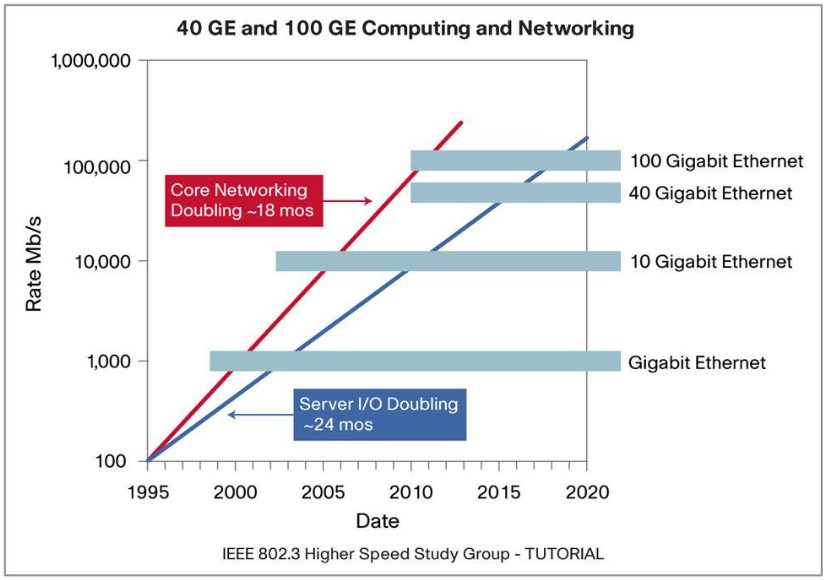
\includegraphics[width=13cm,keepaspectratio]{fig/performance-gap.png}
	\caption{Network and CPU performance gap (source:~\cite{cisco-market-need})}
	\label{fig:40gbe-performance-gap}
	\bigskip
\end{figure}

The 802.3ba standard specifies the physical coding sublayer that is common to both
40 and 100~Gb/s physical layer implementations~\cite{ieee-802.3ba}.
This physical coding sublayer is known as 40GBASE-R and 100GBASE-R.
802.3ba further specifies the following 40~GbE port types.
All of them use 4 fiber pairs and 40GBASE-R physical coding.
\begin{itemize}
\item 40GBASE-SR4 runs over multimode fiber with Short reach for at least 100~m range
\item 40GBASE-LR4 runs over single mode fiber with Long reach, with the required operating range at least 10~km
\item 40GBASE-CR4 is a Copper type over twinaxial cable
\item 40GBASE-KR4 is a port type for bacKplanes
\item 40GBASE-ER4 with an Extended operating range at least 30~km, which
is currently under discussion by the IEEE P802.3bm 40GBASE-ER4 Task Force~\cite{ieee-802.3bm}.
\end{itemize}

The 40GBASE-SR4 runs on Quad (4-channel) Small Form Factor Pluggable (abbreviated as QSPF or QSPF+).
QSPF is a high-density fiber connector with 12 strands of fiber.
Each channel has a dedicated transmit fiber and a dedicated receive fiber.
The middle four fibers remain unused~\cite{cisco-market-need}.
The channel layout is shown in figure~\ref{fig:40gbe-ethernet-layout}.
\begin{figure}
	\centering
	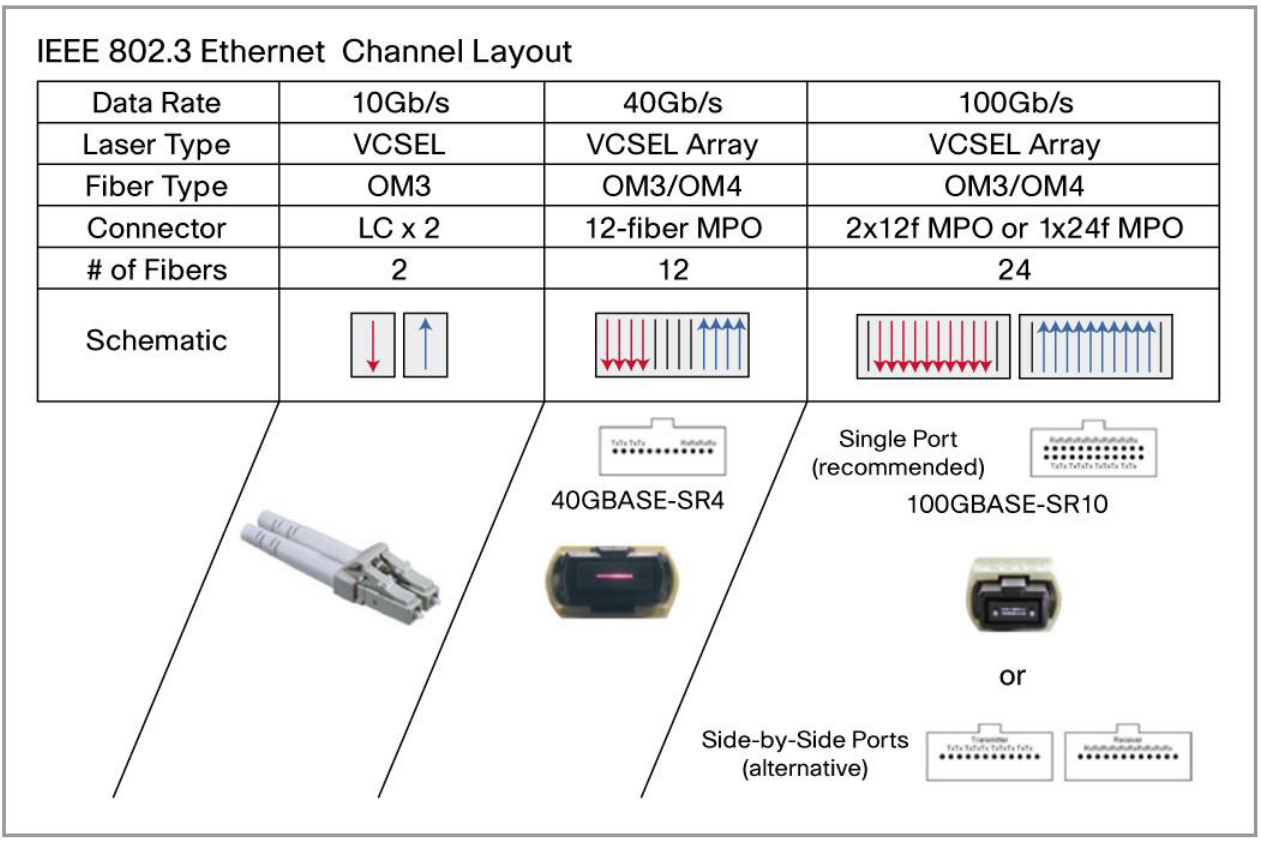
\includegraphics[width=13cm,keepaspectratio]{fig/ethernet-layout.png}
	\caption{IEEE 802.3 Ethernet Channel Layout (source:~\cite{cisco-market-need})}
	\label{fig:40gbe-ethernet-layout}
	\bigskip
\end{figure}

%=========================================================================
% (c) 2014, 2015 Josef Lusticky

\section{Frame rates}\label{sec:40gbe-frame-rates}
At 40 Gigabits per second rate, it takes $\frac{8}{40 \times 10^{9}} = 0.2~ns$ to transfer a single octet.
The time to transfer a whole frame depends on its size.
The standard Ethernet frame size remains unchanged in the IEEE 802.3ba standard and
is between 72 and 1526~octets.
Frames are separated by the Interframe gap (IFG) - a pause between two consecutive frames.
In 40 and 100~Gigabit Ethernet,
the length of IFG may vary due to clock tolerance and lane alignment requirements,
but it must be at least 1 octet.
The mean length of IFG is 12~octets~\cite{ieee-802.3ba}.

Figure~\ref{fig:40gbe-ethernet-frame} shows the Ethernet frame format with no extensions (e.g. 802.1Q VLAN tag).
Each frame starts with an 8-octet Preamble, which consists of a 7-octet pattern of alternating 1 and 0 bits,
and 1 octet of 1010~1011 value called Start of Frame Delimiter~(SFD).
The SFD is designed to break the previous 7-octet pattern and to signal the start of the actual frame~\cite{ieee-802.3ba}.

The Destination MAC address, Source MAC address and Type or Length fields form the link-layer Ethernet header.
The Type or Length field represents Type in case of Ethernet II (DIX) frame
and Length in case of IEEE 802.3 frame.
Both formats are in use today~\cite{understanding-internals}.

The Payload field represents the transferred Layer~3 data of a variable size.
The size of the data is bound by the standard Ethernet frame size and can be up to 1500~octets,
which is the Maximum Transmission Unit (MTU) of Ethernet~\cite{ieee-802.3ba}.
Frame Check Sequence (FCS) is a 4-octet cyclic redundancy code to check the integrity of the received frame.

\begin{figure}
	\centering
	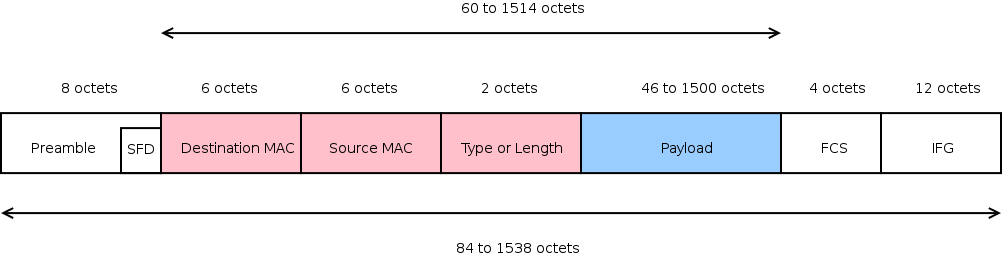
\includegraphics[width=15cm,keepaspectratio]{fig/ethernet-frame.png}
	\caption{Ethernet frame format}
	\label{fig:40gbe-ethernet-frame}
	\bigskip
\end{figure}

The Preamble, FCS and IFG carry no data and provide a necessary overhead of 24~octets for each frame.
The size of this overhead is independent from the Payload size.
Upon arrival of a frame, the rest is transferred from a network adapter to the host CPU and processed.
The data in the Ethernet header (Source and Destination MAC addresses and Type or Length) are used for L2 processing.
The data in the Payload field are used for L3 processing (i.e. routing).

The maximum sized frame is 1538 octets including the Interframe gap
(8-octet Preamble + 14-octet Ethernet header + 1500-octet Payload + 4-octet FCS + 12-octet Interframe gap).
At 40~Gbps rate, a traffic consisting of only the maximum sized frames of 1538 octets
produces $\frac{40 \times 10^{9}}{1538 \times 8} = 3~250~975$ frames per second.
In reference to the minimum frame size of 84~octets including IFG,
the 40~Gigabit Ethernet can transmit up to $\frac{40 \times 10^{9}}{84 \times 8} = 59~523~809$~frames per second.

Since each frame must be processed separately,
such high frame rates require enormous fast processing speed.
Despite the continual frame rates increases,
the 1500 byte Maximum Transmission Unit (MTU) of Ethernet remains unchanged.

Extensions to allow larger frames were made by several vendors.
The typical maximum sized jumbo frames in use are 9~038 octets (carrying 9~000 octets of Payload)~\cite{ea-jumbo-frames}.
The 40~GbE transmits $\frac{40 \times 10^{9}}{9038 \times 8} = 555~555$~of such jumbo frames per second at full rate.


%=========================================================================
% (c) 2014, 2015 Josef Lusticky

\section{Throughput}\label{sec:40gbe-throughput}
With 40~GbE, not only the per frame processing became a concern.
In case of the maximum sized frames,
40~Gbps Ethernet NIC transfers $3~259~452 \times 1514 \doteq 4.6$~GB/s of L2 data
(Ethernet header and Payload) to the host CPU.
Since the frame overhead is independent from its size,
the efficiency of Ethernet drops significantly with smaller frames.
In case of the minimum sized frames, the transfer rate drops to $59~523~809 \times 60 \doteq 2.6$~GB/s
while still operating at 40~Gbps rate.
Such data rates require appropriate bus between the NIC and the CPU to operate at full speed.

A single PCI-Express 2.0 lane provides throughput of 5~Gigatransfers per second in each direction~\cite{pcie-specification}.
In this case, Gigatransfer per second is the same as gigabit per second,
but it also includes the bits that are lost as a result of the interface overhead.
PCI-Express 2.0 uses 8b/10b coding, that is, 8 bits of data cost 10 bits to transfer (the same as in SATA case)~\cite{pcie-bandwidth}.
Therefore, the actual bandwidth is 500~MB/s per lane.
A PCI-Express 2.0 link with 8 lanes provides 4~GB/s throughput,
which is not enough to transfer the 40~GbE traffic between the NIC and the CPU.
The widest 16-lanes link doubles the throughput to 8~GB/s, which is sufficient for a 40~GbE adapter.

PCI-Express 3.0 increases throughput to 8~Gigatransfers/s in each direction for a single lane~\cite{pcie-specification}.
Additionally, it uses more efficient 128b/130b coding.
This way, a bandwidth of 984.6~MB/s per lane is achieved, almost twice the PCI-Express 2.0.
An 8-lane PCI-Express 3.0 link provides 7~876.8~MB/s bandwidth which is sufficient to handle 40~GbE traffic.

The above calculations do not include an additional overhead of the PCI-Express link headers
and signalling interrupts.
The PCI-Express devices are required to support the Message Signalled Interrupts (MSI) feature~\cite{pcie-specification}.
MSI is a technique to generate interrupts by writing to a specified address,
which has been written into the peripheral's configuration during initialisation.
The interrupt signalling consists of sending a Write request over the PCI-Express link
to the specified address~\cite{pcie-tutorial-1}.
There can be up to 32 MSI interrupts assigned to a single device,
but the number of interrupts the device uses must be a power of 2~\cite{msi-driver-guide}.

MSI-X is an extension to the MSI mechanism, which introduces various new features.
MSI-X provides support for signalling an interrupt directly to a particular CPU
and it allows to use up to 2048 interrupts and the number of interrupts is not restricted to a power of 2.
This feature is used by modern 40~GbE adapters to spread
the work related to traffic processing among multiple CPUs.
The device can use either MSI or MSI-X, but not both simultaneously~\cite{msi-driver-guide}.

Although both PCI-Express 2.0 x16 and PCI-Express 3.0 x8 links can be used for 40~GbE cards,
NIC vendors tend to produce 40~GbE PCI 3.0 x8 adapters,
because a PCI-Express x8 adapter can be plugged into a x16 slot, but not the other way round~\cite{pcie-specification}.
An adapter with less lanes saves both costs and troubles finding an empty x16 slot.


%=========================================================================
% (c) 2014, 2015 Josef Lusticky

\section{Compatibility}\label{sec:40gbe-compatibility}
The previous 10~Gigabit Ethernet standard was ratified by the IEEE 802.3 Working Group in 2002~\cite{ieee-802.3ae}.
As opposed to 40~GbE, the cabling plant of 10~GbE uses just a single pair of fiber.
In 2013, Cisco introduced a replacement that does not require a change to the cabling plant
and makes it possible to run 40~GbE over a single pair of multimode fiber~\cite{40gbe-mmf}.

Since its ratification in 2002,
it took four years to standardise 10~GbE over copper twisted pair 10GBASE-T in 2006~\cite{ieee-802.3an}.
10GBASE-T can run over a Category~6 cable within the range of 55m.
For full 100m range, a Category~6a cable is required~\cite{ieee-802.3an}.
One of the previous barriers to 10GBASE-T adoption was the power consumption per port compared to other 10 GbE options.
However, improvements in semiconductor manufacturing technology
significantly decreased power use to the point where it is no longer a concern.
Nowadays, 10GBASE-T and Category~6A cabling costs less than optical fiber technology~\cite{belden-10g-40g}.

The 40~GbE over Category~8 copper twisted pair
is currently being discussed by the IEEE P802.3bq 40GBASE-T Task Force.
The maximum range for 40GBASE-T is planned to be just 30 meters~\cite{ieee-802.3bq}.
Such range should be sufficient for most switch-to-server connections in data centres.
Because of the shorter distance, the power consumption of 40GBASE-T should be less than of 10GBASE-T~\cite{belden-10g-40g}.

40~Gigabit Ethernet is backward compatible with its predecessor.
Due to concerns around vendor and equipment interoperability,
IEEE has determined they will not support or define Jumbo frames~\cite{ea-jumbo-frames}.
Modern 100Mbps or higher Ethernet also uses constant signalling, which avoids the need for the preamble~\cite{anatomy-frame}.
However, the frame format is preserved for today's Ethernet transmission speeds to avoid making any changes.
With the upcoming 40GBASE-T variant, 10M/100M/1G/10G/40G link speed auto-negotiation can be expected in the future.

The 40~Gigabit Ethernet protocol support was introduced in the Linux kernel by various NIC vendors.
Red Hat Enterprise Linux 7 supports 40 Gigabit network interface controllers since its initial release~\cite{rhel-7-announce}.
Additional support was also introduced in RHEL 6.6~\cite{rhel-66-announce}.



%=========================================================================
% (c) 2014, 2015 Josef Lusticky

\chapter{Linux Kernel Packet Processing}

Linux version 3.10 consists of nearly 17 million lines of code.
http://www.cnet.com/news/linux-development-by-the-numbers-big-and-getting-bigger/

Processing packets in the Linux kernel.
There are two modes of processing packets from NIC.
The traditional way is interrupt-driven - each incomming packet is an
asynchronous event which causes interrupt.

The poll method introduced in the New API (NAPI) - only the first incomming packet causes interrupt
and other packets are polled.
NAPI is designed to improve the performance of high-speed networking.
The driver using NAPI provides the poll function to the kernel for reading received packets.

Most of the new drivers support this feature.
When under a heavy load, the packets are lost because of not enough space in NIC buffer.
The packets to be lost are not fed into the network stack, so they take no CPU time.
http://www.haifux.org/lectures/172/netLec.pdf


TCP Segment Offload - kernel is not dealing with segmenting.
ethtool -K eth1 tso on
ethtool -k eth1


\section{NAPI}

NAPI is a proven (www.cyberus.ca/~hadi/usenix-paper.tgz) technique
to improve network performance on Linux.
http://lwn.net/2002/0321/a/napi-howto.php3
---

NAPI ("New API", though it is not so new anymore, since linux kernel 2.6) is an extension to the device driver packet processing framework, which is designed to improve the performance of high-speed networking~\cite{linux-foundation-napi}.

NAPI works through:

Interrupt mitigation 
    High-speed networking can create thousands of interrupts per second, all of which tell the system something it already knew: it has lots of packets to process. NAPI allows drivers to run with (some) interrupts disabled during times of high traffic, with a corresponding decrease in system load.

Packet throttling 
    When the system is overwhelmed and must drop packets, it's better if those packets are disposed of before much effort goes into processing them. NAPI-compliant drivers can often cause packets to be dropped in the network adaptor itself, before the kernel sees them at all.

More careful packet treatment, with special care taken to avoid reordering packets. Out-of-order packets can be a significant performance bottleneck. 


NAPI additions to the kernel do not break backward compatibility and drivers may still process completions directly in interrupt context if necessary.

http://lwn.net/Articles/30107/

-----


NAPI is an interrupt mitigation mechanism used with network devices. When network traffic is heavy, the kernel can safely predict that incoming packets will be available anytime it gets around to looking, so there is no need to have the adapter interrupting it (possibly thousands of times per second) to tell it about those packets. So a NAPI-compliant driver will turn off the packet receive interrupt and provide a poll() method to the kernel. When the kernel is ready to deal with more packets, poll() will be called with a maximum number of packets it is allowed to feed into the kernel; it should process up to that many packets and quit.
http://lwn.net/Articles/214457/

-----

Network interfaces, like most reasonable peripheral devices, are capable of interrupting the CPU whenever a packet arrives. But even a moderately busy interface can handle hundreds or thousands of packets per second; per-packet interrupts would quickly overwhelm the processor with interrupt-handling work, leaving little time for getting useful tasks done. So most interface drivers will disable the per-packet interrupt when the traffic level is high enough and, with cooperation from the core networking stack, occasionally poll the device for new packets. There are a number of advantages to doing things this way: vast numbers of interrupts can be avoided, incoming packets can be more efficiently processed in batches, and, if packets must be dropped in response to load, they can be discarded in the interface before they ever hit the network stack. Polling is thus a win for almost all situations where there is any significant amount of traffic at all. 
http://lwn.net/Articles/551284/

---

NAPI is pretty good, but optimized for throughput

Latency is high by default (especially for Ethernet)
Jitter is unpredictable by default

netperf

http://www.linuxplumbersconf.org/2012/wp-content/uploads/2012/09/2012-lpc-Low-Latency-Sockets-slides-brandeburg.pdf

----

It is also possible to use NAPI in wireless 802.11 drivers.


%=========================================================================
% (c) 2014, 2015 Josef Lusticky

\chapter{Analysis}\label{chap:analysis}
Basically, there are three important parts needed to perform network benchmarks at full 40 Gbit speed -
a network interface card with 40~Gigabit Ethernet support, a server compatible with the card and a packet generator
capable of generating 40~Gbps network traffic.
A chosen distribution of the GNU/Linux operating system should contain a stable and
recent kernel that supports the 40~Gb Ethernet protocol, the network interface card
and the features described in chapter~\ref{chap:linux}.

%=========================================================================
% (c) 2014, 2015 Josef Lusticky

\section{Hardware and networking}\label{sec:setup-hardware}
Figure~\ref{fig:setup-supermicro-board} shows the block diagram of the Supermicro motherboard.
The Intel Xeon E5-2660 v2 processors were plugged into the CPU sockets.
The Mellanox ConnectX-3 EN adpater was plugged into the PCIE 3.0 x8 Upper slot,
which is part of the {\it{WIO}} block.
The PCI-Express links are directly connected to the CPU~1 only.
\begin{figure}
	\centering
	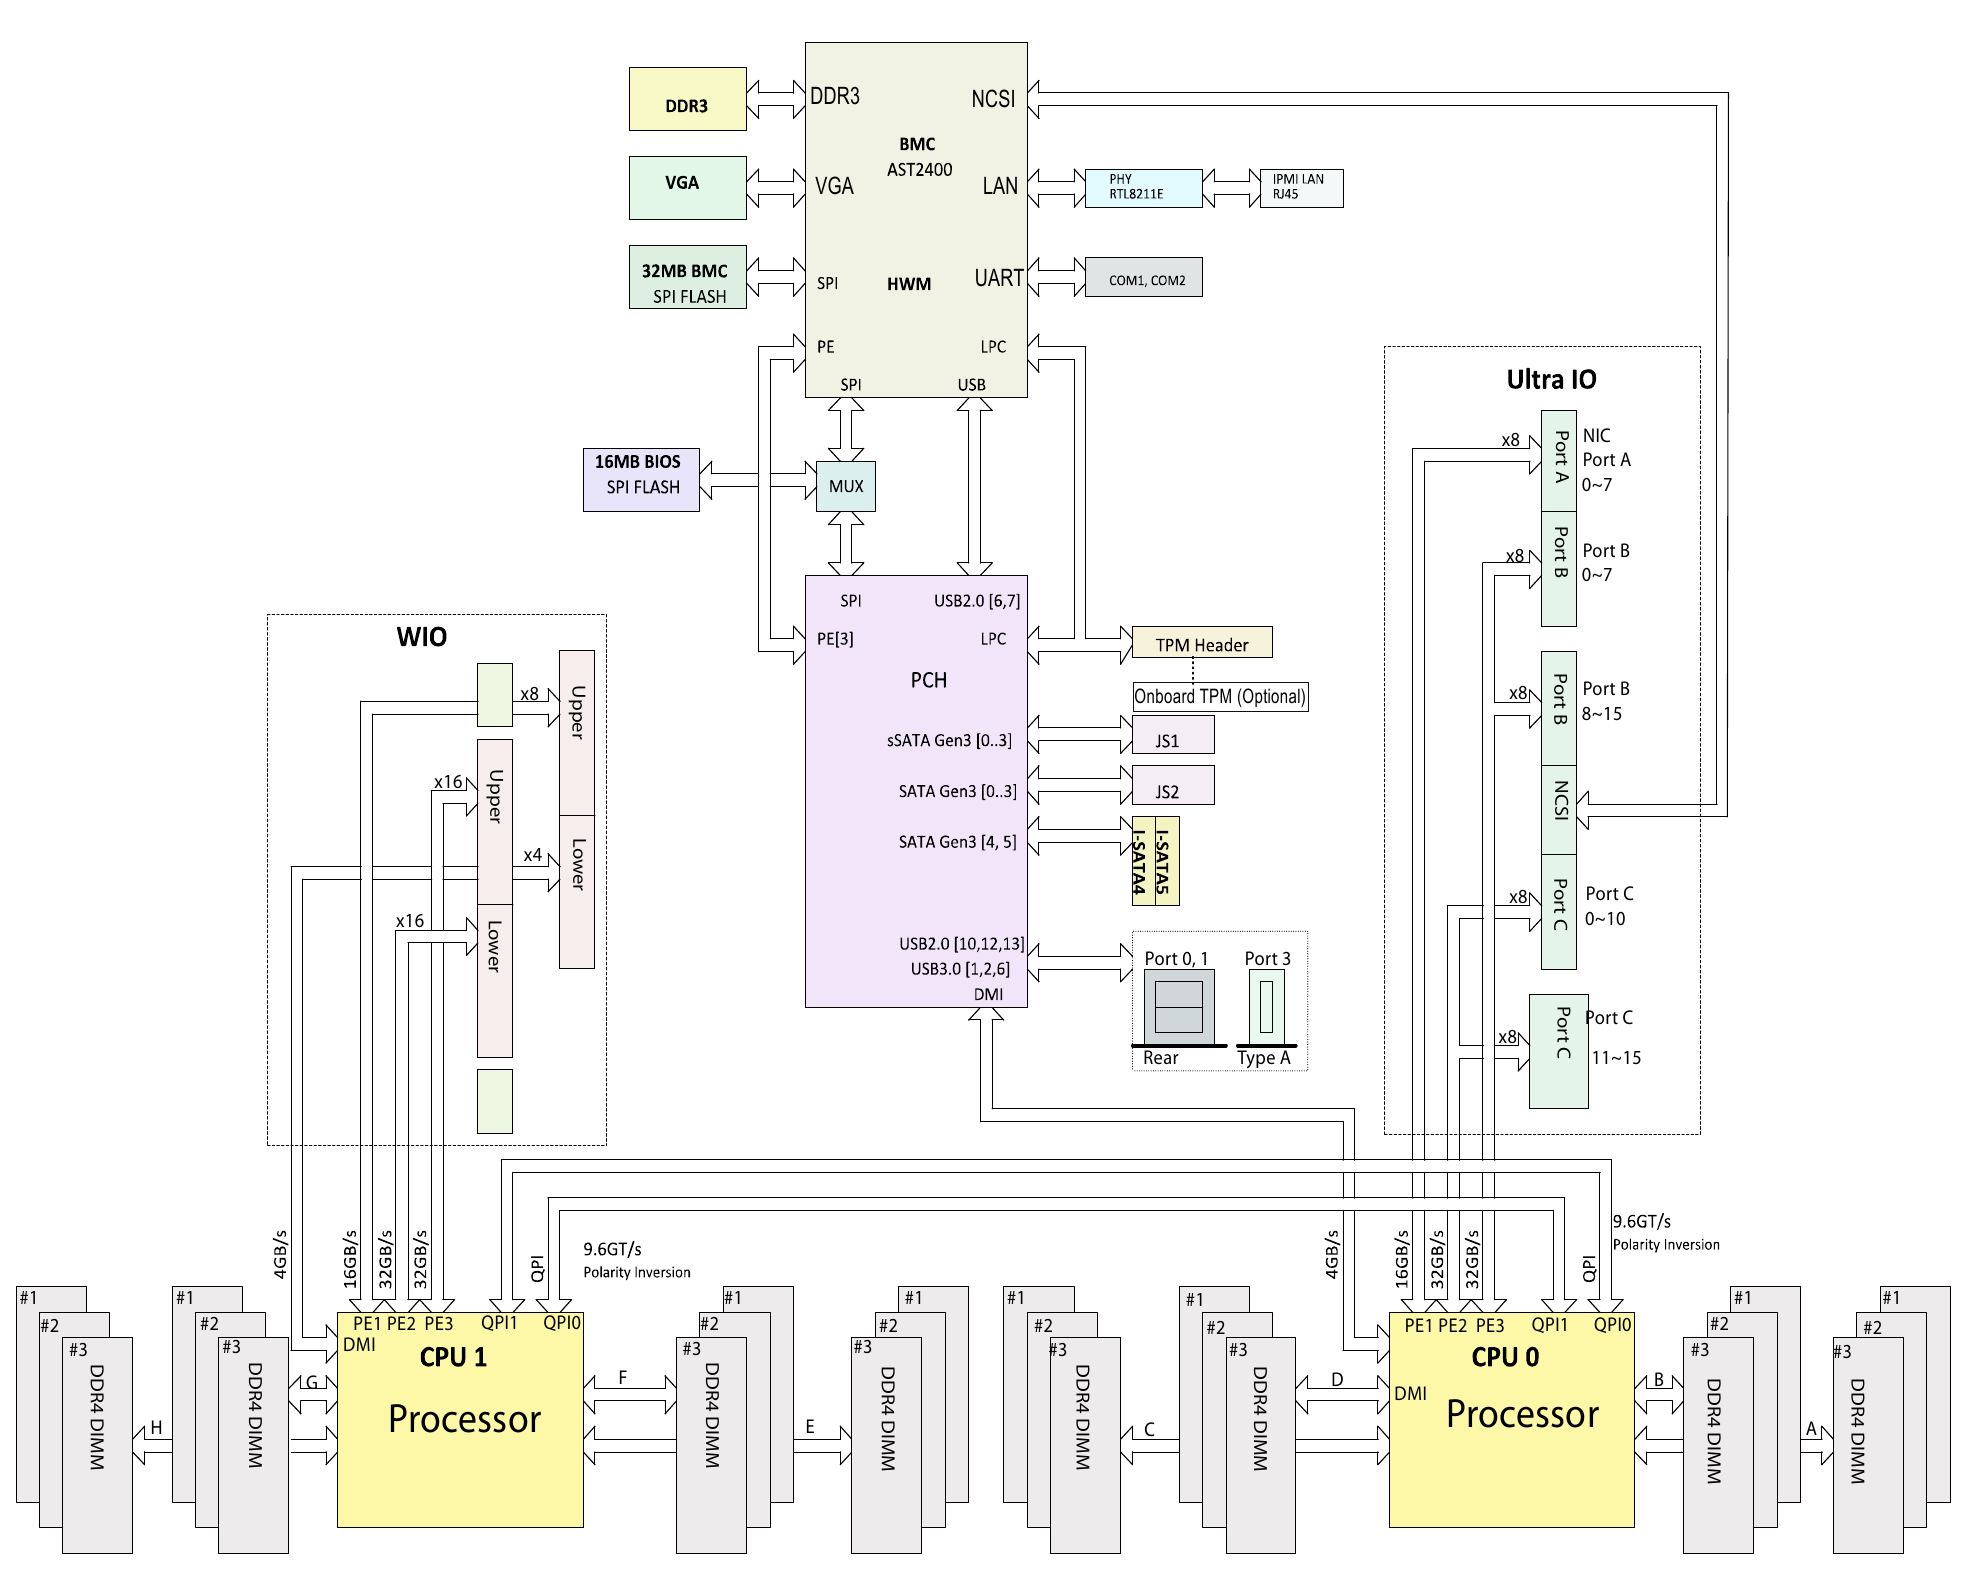
\includegraphics[width=15cm,keepaspectratio]{fig/supermicro-x10drui.png}
	\caption{Supermicro motherboard's block diagram}
	\label{fig:setup-supermicro-board}
\end{figure}

The server was put to the same rack as the Spirent hardware generator.
A pair of 40GBASE-SR4 multimode fiber cables with QSPF connectors
was used to connect Spirent with the Mellanox ConnectX-3 EN adapter.

IPv4 addresses from 192.0.2.0/24 (TEST-NET-1) block were assigned~\cite{rfc5737}.
IPv6 addresses from 2001:db8::/32 range were assigned.
Addresses within these blocks should not appear on the public Internet~\cite{rfc3849}.
Figure~\ref{fig:addressing-scheme} shows the addressing scheme used for the measurements.
\begin{figure}[H]
	\centering
	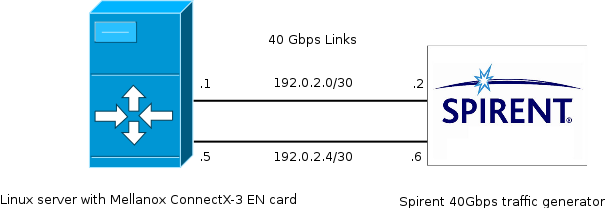
\includegraphics[width=13.5cm,keepaspectratio]{fig/net-setup.png}
	\caption{Addressing scheme}
	\label{fig:addressing-scheme}
\end{figure}



%Enable IPv4 packet forwarding:
%echo 1 > /proc/sys/net/ipv4/ip\_forward


%ip neigh add 1.0.0.2 lladdr f4:52:14:5e:6c:71 dev enp6s0d1
%ip neigh add 2.0.0.2 lladdr f4:52:14:5e:6c:70 dev enp6s0

%ip addr add 1.0.0.1/24 broadcast 1.0.0.255 dev enp6s0d1
%ip addr add 2.0.0.1/24 broadcast 2.0.0.255 dev enp6s0


%Load BGP routes:
%\begin{lstlisting}
%Basic info: size of leaf: 40 bytes, size of tnode: 40 bytes.
%Main:
        %Aver depth:     2.43
        %Max depth:      8
        %Leaves:         503308
        %Prefixes:       538739
        %Internal nodes: 114430
          %1: 58725  2: 26171  3: 14808  4: 7316  5: 4239  6: 2103  7: 1065  8: 2  17: 1
        %Pointers: 995798
%Null ptrs: 378061
%Total size: 61373  kB
%\end{lstlisting}


%=========================================================================
% (c) 2014, 2015 Josef Lusticky

\section{Software and firmware}
Base CentOS 7 was installed on the server.
The operating system features Linux kernel based on version 3.10 -
the installed version is 3.10.0-123.20.1.el7.x86\_64.
The operating system was updated with all updates available as of 1st May 2015.
The upstream kernel version 4.0.2 was additionally installed from the ELRepo repository~\cite{elrepo-kernel-ml}.

The Linux kernel detects the Mellanox ConnectX-3 EN card automatically and loads the mlx4\_core and mlx4\_en module.
The mlx4\_core module prints the detected PCI-Express link parameters to the kernel's message buffer.
The buffer can be viewed using the {\it{dmesg}} utility and its partial output is shown bellow:
\begin{lstlisting}[language=TeX]
mlx4_core 0000:06:00.0: PCIe link speed is 8.0GT/s, device supports 8.0GT/s
mlx4_core 0000:06:00.0: PCIe link width is x8, device supports x8
\end{lstlisting}
The mlx4\_core module further registers interrupts and prints the assigned IRQ numbers for each queue
to the kernel's message buffer:
\begin{lstlisting}[language=TeX]
mlx4_core 0000:06:00.0: irq 61 for MSI/MSI-X
mlx4_core 0000:06:00.0: irq 62 for MSI/MSI-X
...
mlx4_core 0000:06:00.0: irq 90 for MSI/MSI-X
\end{lstlisting}

The driver uses either MSI or MSI-X feature of the PCI-Express bus, as described in section~\ref{sec:40gbe-throughput}.
The MSI-X feature is used automatically if the system supports it, otherwise the adapter uses MSI.
The {\it{lspci -vv}} command can be used to check whether MSI-X is used.
Listing~\ref{lst:setup-lspci} shows partial output of lspci for the Mellanox ConnectX-3 EN adapter.
The MSI-X capability is followed by an Enable flag which is followed with either "+" (enabled)
or "-" (disabled).
Listing~\ref{lst:setup-lspci} shows that the system supports MSI-X and the adapter is configured to use it.
\begin{lstlisting}[language=TeX,label={lst:setup-lspci},caption={Partial output of lspci -vv for Mellanox ConnectX-3 EN}]
06:00.0 Ethernet controller: Mellanox Technologies MT27500 Family [ConnectX-3]
		...
		Capabilities: [9c] MSI-X: Enable+ Count=128 Masked-
				...
				LnkCap: Port #8, Speed 8GT/s, Width x8, ASPM L0s, Exit Latency L0s unlimited, L1 unlimited
				...
\end{lstlisting}

Apart from the NIC driver, the Mellanox ConnectX-3 adapter uses its own proprietary firmware.
The firmware was updated to version 2.32.5100, which is the latest version available as of 10th January 2015.
The firmware is not part of the Linux kernel and its update procedure is described in appendix~\ref{app:firmware}.


%=========================================================================
% (c) 2014, 2015 Josef Lusticky

\section{Benchmarking methodology}\label{sec:analysis-metodology}
Procedures described by RFC~2544 can be used to measure routing performance of the Linux kernel.
RFC~2544 specifies the benchmarking methodology for network interconnect devices.
The ideal way to implement the series of tests described in RFC~2544 is to use a tester
with both transmitting and receiving ports.
Connections are made from the sending ports of the tester to the receiving ports of the
device under test (DUT) and from the sending ports of the DUT back to the tester~\cite{rfc2544}.
Figure~\ref{fig:analysis-rfc2544} shows the test implementation.

Since the tester both sends the test traffic and receives
it back, after the traffic has been forwarded by the DUT, the tester
can easily determine if all of the transmitted packets were received~\cite{rfc2544}.
The Spirent TestCenter Application provides statistics about transmitted and received frames,
which can be used for this purpose.
\begin{figure}
	\centering
	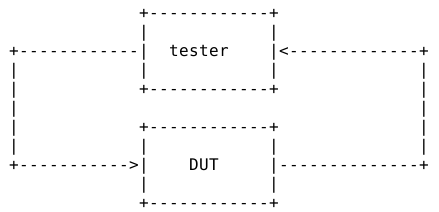
\includegraphics[width=9cm,keepaspectratio]{fig/rfc2544.png}
	\caption{RFC2544 test implementation (source:~\cite{rfc2544})}
	\label{fig:analysis-rfc2544}
\end{figure}

\input{analysis/metodology-generation.tex}

\input{analysis/metodology-collection.tex}


%=========================================================================
% (c) 2014, 2015 Josef Lusticky

\section{Software settings}\label{sec:analysis-settings}
The CentOS 7 operating system features various components that influence forwarding performance.
To measure a pure routing performance of the Linux kernel,
the Netfilter and SELinux components should be disabled.
If disabling the netfilter is not appropriate, the iptables utility must be used to configure netfilter to allow forwarding,
because the default rules do not allow packet forwarding.
SELinux in the CentOS~7 operating system uses enforcing policy by default.
Similarly to netfilter, the SELinux component should be disabled to prevent performance decrease.
Influence of both the components on forwarding performance can be measured.

The Linux kernel features dynamic CPU frequency scaling.
The CPUFreq governors are policies that decide what frequency should be used.
The CPUfreq governor {\it{performance}} should be used during the measurements, as it sets the CPU statically to the
highest frequency avaliable~\cite{cpufreq-governors}. %, which is 2.6~GHz in case of Intel Xeon E5-2630 v2.

Packet processing by the Linux kernel can be configured in different ways.
To change the Linux kernel compile-time configuration, the kernel must be recompiled.
The CentOS~7 kernel provides a fair amount of features that could break existing setups when disabled.
The default kernel compile-time configuration does not have to provide the best routing performance,
however, it is usually used in most scenarious and hence its benchmark results are of interests for most people.
The features configured during compile-time of the Linux kernel introduce
just a negligible overhead when they are not used.
For example, the MULTIPLE\_IP\_TABLES support is enabled in the CentOS 7 distribution kernel, however,
since the measurements presented in this thesis use no policy routing,
the FIB lookup principle described in section~\ref{sec:linux-routing} is still performed.

Apart from compile-time options, the Linux kernel configuration can be changed during run-time.
The proc and sys filesystems provide access to the kernel variables that influence packet processing.
Tuning of these variables can provide significant amount of routing performance improvement when configured properly.

\subsection{Procfs settings}
The variables exported via procfs are accessible in CentOS~7 as read-write files in /proc.
The variables in the /proc/sys directory can be changed by the sysctl utility as well.
The files in the /proc/sys/net directory are of interest for the experiments.
This directory includes the following subdirectories:
\begin{itemize}
\item /proc/sys/net/ipv4 - variables influencing the IPv4 protocol settings
\item /proc/sys/net/ipv6 - variables influencing the IPv6 protocol settings
\item /proc/sys/net/netfilter - variables influencing the netfilter settings, not discussed in this thesis
\item /proc/sys/net/unix - variables influencing communication over unix sockets, not discussed in this thesis
\item /proc/sys/net/core - variables influencing low-level network settings, including parameters of NAPI, Low Latency Sockets, etc.
\end{itemize}

The most important setting for the routing performance measurements of the Linux kernel is IPv4 forwarding.
It can be enabled by writing "1" to the /proc/sys/net/ipv4/ip\_forward file.
This variable is special - its change resets all IPv4 configuration parameters to their default state~\cite{kernel-doc-ip-sysctl}.
The /proc/sys/net/ipv4/conf/{\it{ifname}}/forwarding file can be used
to further selectively enable or disable forwarding on a particular interface.
Historically, some of the files in /proc/sys/net/ipv4 also influence settings of L4 protocols.
Although these files are located in the ipv4 subdirectory, the L4 settings are independent on the underlying protocol.

Files in the ipv6 directory influence the IPv6 protocol settings only.
The IPv6 protocol is disabled in CentOS 7 on all interfaces by default.
The variable accessible via /proc/sys/net/ipv6/conf/all/disable\_ipv6 must be changed to "0" to
enable the IPv6 protocol on all interfaces.
Similarly, the /proc/sys/net/ipv6/conf/all/forwarding variable must changed to "1" to enable IPv6 forwarding on all interfaces.
Both settings can be changed on per-interface basis as well.

The /proc/sys/net/ipv4/route.max\_size sets the maximum number of IPv4 routes allowed in the kernel.
This is 2~147~483~647 by default in CentOS~7, which is enough for a full BGP table,
which contains approx.~538~000 prefixes at the time of writing. %TODO cite
The /proc/sys/net/ipv6/route.max\_size sets the maximum number of IPv6 routes allowed in the kernel.
This is 4096 by default in CentOS~7, which must be raised for the measurements involving BGP routes.
The number of IPv6 prefixes announced in the Internet is approx.~22~000 at the time of writing. %TODO cite

The source IPv4 address validation is enabled by default in CentOS 7.
This feature is called Reverse path filtering (rp\_filter) in the Linux kernel and it prevents IP spoofing.
However, it introduces additonal processing and thus it should be disabled during the experiments.
The rp\_filter can be disabled on a particular interface
by writing "0" to /proc/sys/net/ipv4/conf/{\it{ifname}}/rp\_filter~\cite{kernel-doc-ip-sysctl}.
The rp\_filter for IPv6 was implemented in the netfilter subsystem of the Linux kernel and
thus it can be configured by iptables~\cite{kernel-source}.

Files in core directory provide access to low-level variables of the networking code.
There are two parameters that influence NAPI processing.
The /proc/sys/net/core/dev\_weight file sets the maximum number of packets that a single device
can feed to the kernel in its {\it{poll()}} function.
The default value is 64 in CentOS 7.
This value can be increased to allow the device to feed more packets at once.
However, most of the drivers provide their own limit which cannot be overwritten unless the code of the driver is changed.
This is the case of the mlx4 driver as well~\cite{kernel-source}.
The /proc/sys/net/core/netdev\_budget file sets the
maximum number of packets taken from all interfaces by a single {\it{net\_rx\_action()}} run.
The interfaces which are registered to polling are
probed in a round-robin manner, as described in subsection~\ref{subsec:linux-ingress-napi}.
To allow the kernel to spend more time on packet processing, the netdev\_budget value can be increased.

Apart from settings, the proc filesystem provides access to several statistics as well.
The network statistics exported via proc filesystem can be found in the /proc/net directory.
The files in this directory are read-only and cannot be manipulated using the sysctl utility.
There are 2 important files for the measurements - the fib\_trie and fib\_triestat.
The fib\_trie file exports the kernel's Forwarding Information Base overview.
The file describes both the Main and Local FIBs, as described in section~\ref{sec:linux-routing}.
The fib\_triestat file exports metadata of the FIB trie structures,
such as average depth, maximum depth, number of leaves, etc.

\subsection{Sysfs settings}
Apart from the proc filesystem, the Linux kernel provides another virtual filesystem found in /sys.
Every interface is represented by a symlink in the /sys/class/net/ directory.
The symlinks point to the corresponding network device, which is represented as a directory in sysfs.

The scaling mechanisms described in section~\ref{sec:linux-scaling} can be set
using files exported in /sys/class/net/{\it{ifname}}/queues.
Each rx-{\it{xx}} subdirectory represents a single hardware receive queue.
The rx-{\it{xx}}/rps_cpus file can be used to set a mask of CPUs serving the particular queue.
Since the Mellanox ConnectX-3 NIC supports RSS, the RPS feature is disabled by default.

%XPS

The sysfs further exports information about loaded modules, including the parameters if a particular module takes any.
The /sys/modules/mxl4\_core/parameters directory contains parameters used by the mlx4\_core module.
The msi\_x parameter is set to 1 by default, which means attempt to use MSI-X.
The /sys/modules/mxl4\_en/parameters directory contains parameters used by the mlx4\_en module.
The udp\_rss parameter is set to 1 by default, which enables RSS for incoming UDP traffic.
There are more parameters taken by both modules, but they are not discussed in this thesis.
Further description of the parameters can be found
in the drivers/net/ethernet/mellanox/mlx4 directory of the Linux kernel source code~\cite{kernel-source}.

\subsection{Ethtool settings}
Ethernet devices can be also configured using ethtool.
Ethtool is a standard Linux utility for controlling network drivers and hardware, particularly for
wired Ethernet devices.
Supported offload features can be displayed using ethtool -{}-show-offload {\it{devname}}.
Listing~\ref{lst:analysis-ethtool-offload} shows output of ethtool -{}-show-offload eth0,
where eth0 is the Mellanox ConnectX-3 adpater.

\begin{lstlisting}[caption={Output of ethtool -{}-show-offload for Mellanox ConnectX3 adapter},label={lst:analysis-ethtool-offload}]
rx-checksumming: on
tx-checksumming: on
	tx-checksum-ipv4: on
	tx-checksum-ip-generic: off [fixed]
	tx-checksum-ipv6: on
	tx-checksum-fcoe-crc: off [fixed]
	tx-checksum-sctp: off [fixed]
scatter-gather: on
	tx-scatter-gather: on
	tx-scatter-gather-fraglist: off [fixed]
tcp-segmentation-offload: on
	tx-tcp-segmentation: on
	tx-tcp-ecn-segmentation: off [fixed]
	tx-tcp6-segmentation: on
udp-fragmentation-offload: off [fixed]
generic-segmentation-offload: on
generic-receive-offload: on
large-receive-offload: off [fixed]
rx-vlan-offload: on [fixed]
tx-vlan-offload: on [fixed]
ntuple-filters: off [fixed]
receive-hashing: on
highdma: on [fixed]
rx-vlan-filter: on [fixed]
vlan-challenged: off [fixed]
tx-lockless: off [fixed]
netns-local: off [fixed]
tx-gso-robust: off [fixed]
tx-fcoe-segmentation: off [fixed]
tx-gre-segmentation: off [fixed]
tx-ipip-segmentation: off [fixed]
tx-sit-segmentation: off [fixed]
tx-udp_tnl-segmentation: off [fixed]
tx-mpls-segmentation: off [fixed]
fcoe-mtu: off [fixed]
tx-nocache-copy: on
loopback: off
rx-fcs: off [fixed]
rx-all: off [fixed]
tx-vlan-stag-hw-insert: off [fixed]
rx-vlan-stag-hw-parse: off [fixed]
rx-vlan-stag-filter: off [fixed]
\end{lstlisting}

Selected offload features can be enabled by issuing ethtool -{}-offload {\it{devname}} {\it{feature}} on,
or disabled by issuing ethtool -{}-offload {\it{devname}} {\it{feature}} off.
The features listed as [fixed] cannot be changed on this paricular NIC.
The rest of the features can be changed, but the feature name differs when issuing ethtool -{}-offload.
For example, the rx-checksumming feature is turned on by issuing ethtool -{}-offload eth0 rx on.
Similarly, the scatter-gather feature is turned on by ethtool -{}-offload eth0 sg on.
For more information about using ethtool, the man page of ethool(8) should be consulted.

Listing~\ref{lst:analysis-ethtool-offload} shows that all supported offload features that are not [fixed], are enabled.


%Interrupt coalescence tunning:
%-C eth0 rx-usecs 50

%Ring buffer tunning:
%-G eth0 rx 1024

%\subsection{Neighboring}
%The destination link layer address must be present in the ARP cache to avoid aditional delay of packet transmission.
%The description of the neighboring implementation is outside the scope of this thesis.
%The amount of ARP and Neighbor Discovery messages is negligible compared to the
%amount of the actual traffic and it is not considered by the measurements.
%However, their processing is not.


%MLX4 driver -  mlx4_en_add - rounddown_pow_of_two
% num_tx_rings_p_up , MLX4_EN_MAX_TX_RING_P_UP
% pocet_TX_rings = pocet_cpu * pocet_RX_rings


TX,RX RING buffer sizes:
Bufferbloat is a phenomenon in packet-switched networks generally,
in which excess buffering of packets causes high latency and packet delay variation (also known as jitter),
as well as reducing the overall network throughput.
When a router device is configured to use excessively large buffers,
even very high-speed networks can become practically unusable for many interactive applications like voice calls,
chat, and even web surfing. %cite http://en.wikipedia.org/wiki/Network_scheduler





%When the Linux kernel is compiled with support for symmetric multiprocessing
%(SMP) and runs on a multiprocessor system, the code for receiving and
%transmitting packets takes full advantage of that power~\cite{understanding-internals}.

%Frames forwarded can be dropped for variety of reasons - no memory in input queue, no mmory in the output queue,
%no route to destination, failed sanity checks, etc~\cite{understanding-internals}.


%Note that ip route show displays the main table.
%For displaying the local table, you should run ip route show table local~\cite{linux-kernel-networking}.





%TODO - describe BGP


%=========================================================================
% (c) 2014, 2015 Josef Lusticky

\chapter{Setup}\label{chap:setup}

%=========================================================================
% (c) 2014, 2015 Josef Lusticky

\section{Hardware and networking}\label{sec:setup-hardware}
Figure~\ref{fig:setup-supermicro-board} shows the block diagram of the Supermicro motherboard.
The Intel Xeon E5-2660 v2 processors were plugged into the CPU sockets.
The Mellanox ConnectX-3 EN adpater was plugged into the PCIE 3.0 x8 Upper slot,
which is part of the {\it{WIO}} block.
The PCI-Express links are directly connected to the CPU~1 only.
\begin{figure}
	\centering
	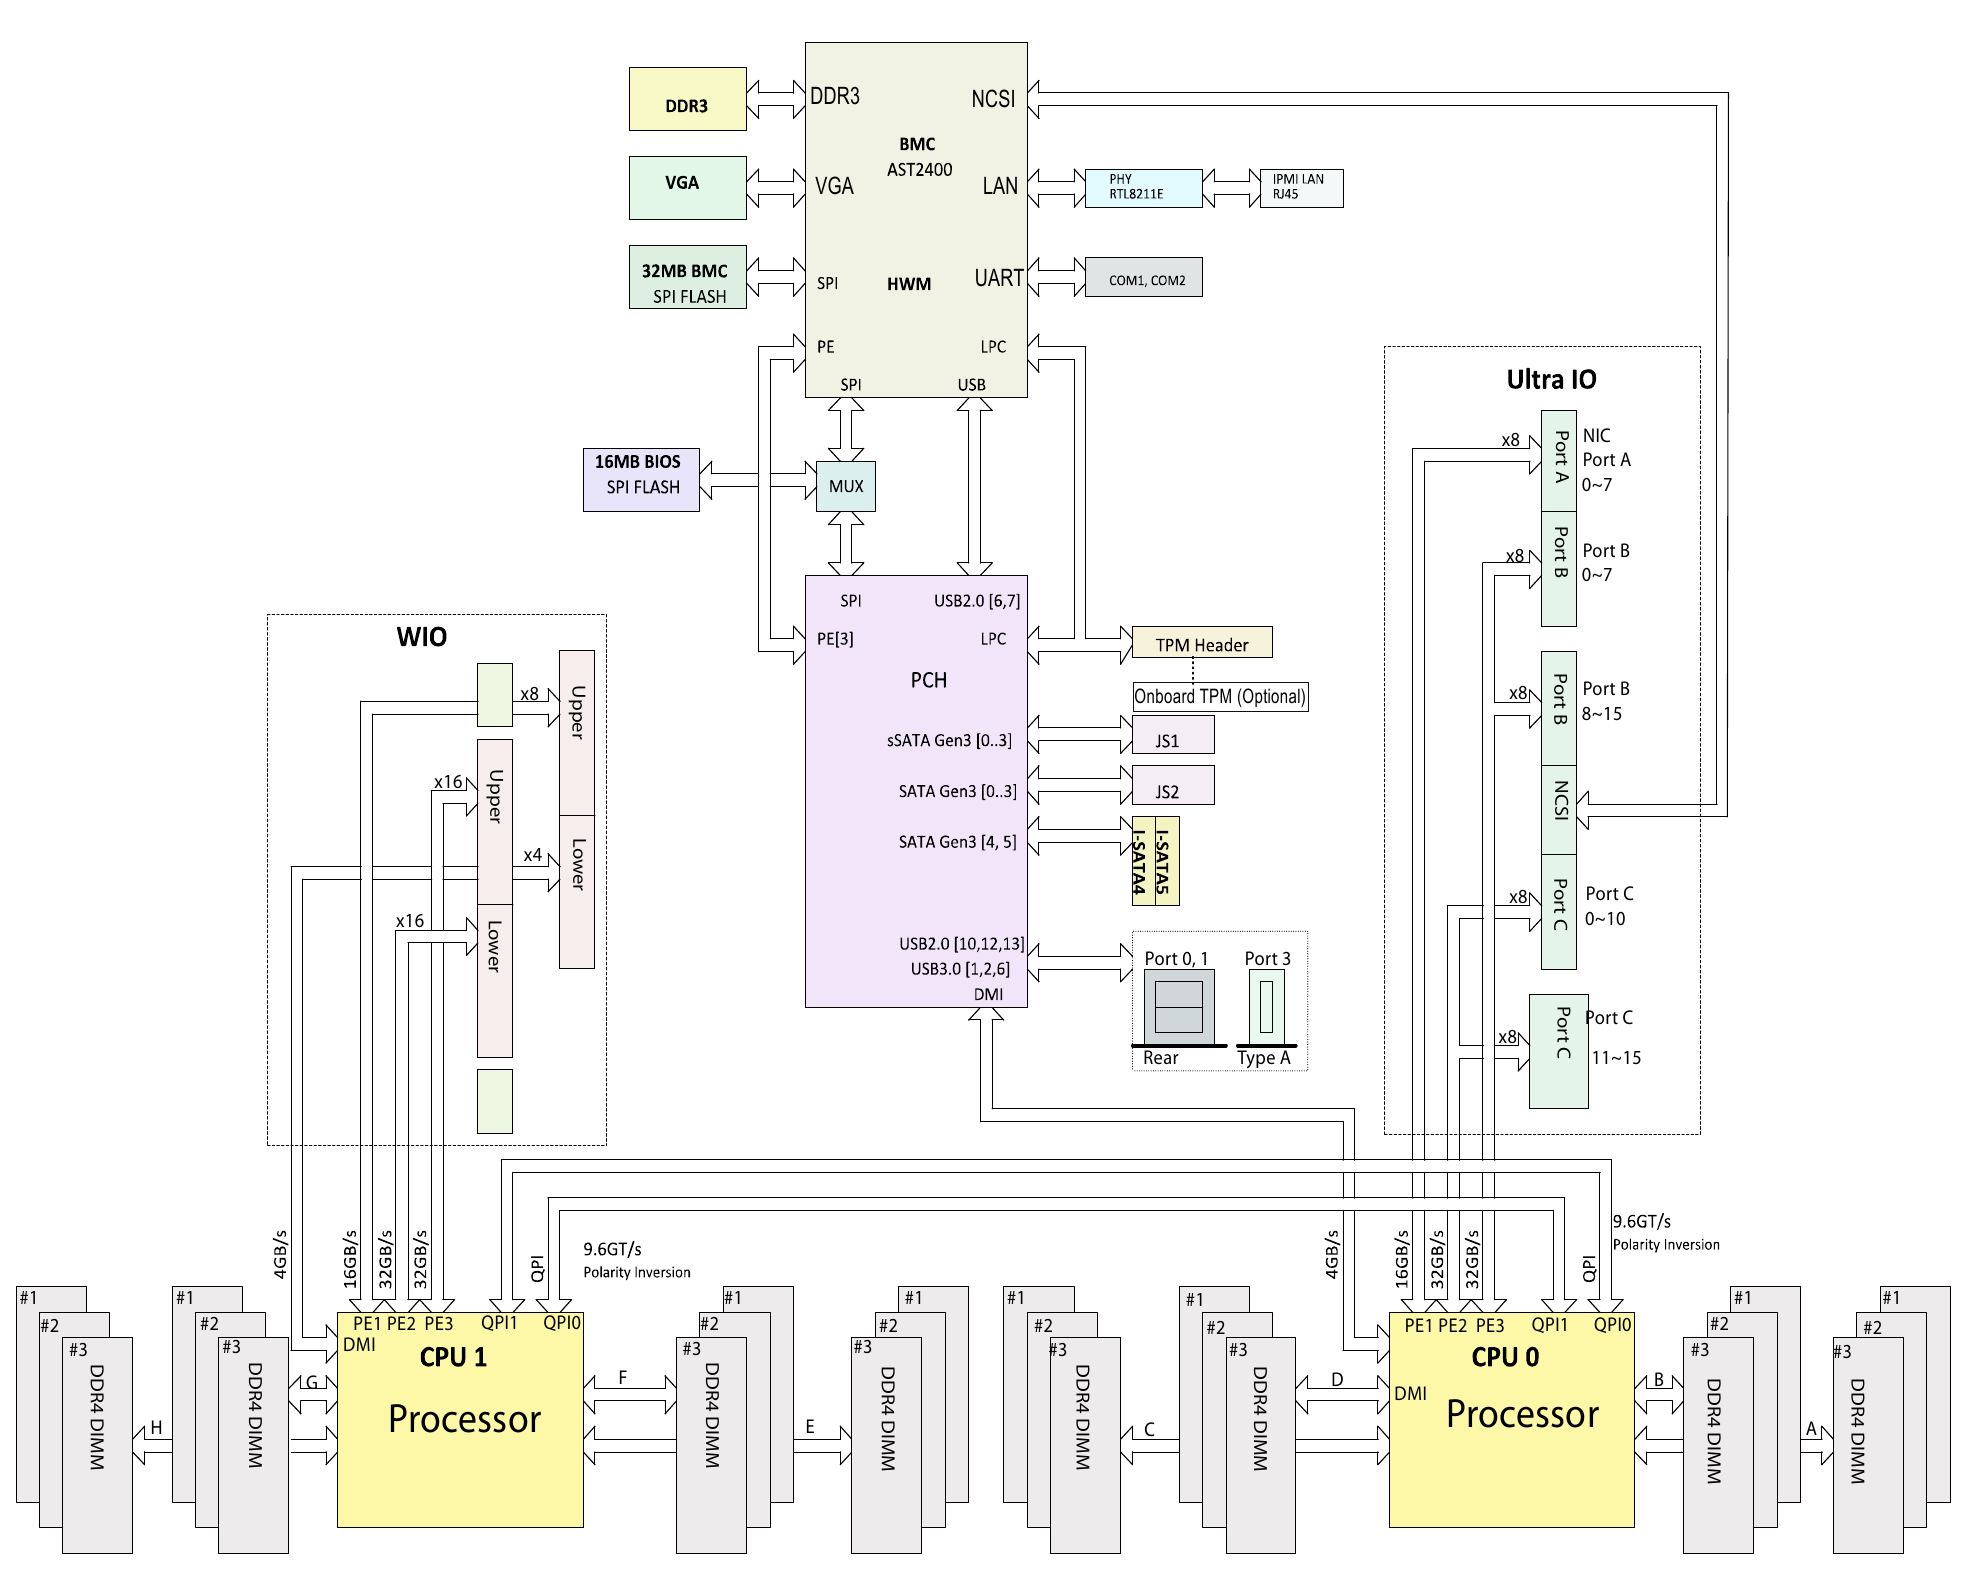
\includegraphics[width=15cm,keepaspectratio]{fig/supermicro-x10drui.png}
	\caption{Supermicro motherboard's block diagram}
	\label{fig:setup-supermicro-board}
\end{figure}

The server was put to the same rack as the Spirent hardware generator.
A pair of 40GBASE-SR4 multimode fiber cables with QSPF connectors
was used to connect Spirent with the Mellanox ConnectX-3 EN adapter.

IPv4 addresses from 192.0.2.0/24 (TEST-NET-1) block were assigned~\cite{rfc5737}.
IPv6 addresses from 2001:db8::/32 range were assigned.
Addresses within these blocks should not appear on the public Internet~\cite{rfc3849}.
Figure~\ref{fig:addressing-scheme} shows the addressing scheme used for the measurements.
\begin{figure}[H]
	\centering
	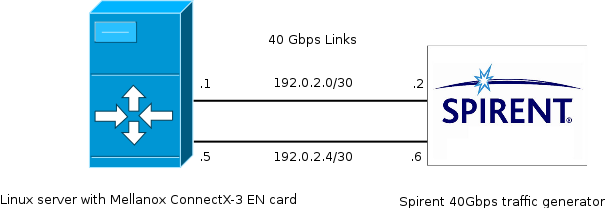
\includegraphics[width=13.5cm,keepaspectratio]{fig/net-setup.png}
	\caption{Addressing scheme}
	\label{fig:addressing-scheme}
\end{figure}



%Enable IPv4 packet forwarding:
%echo 1 > /proc/sys/net/ipv4/ip\_forward


%ip neigh add 1.0.0.2 lladdr f4:52:14:5e:6c:71 dev enp6s0d1
%ip neigh add 2.0.0.2 lladdr f4:52:14:5e:6c:70 dev enp6s0

%ip addr add 1.0.0.1/24 broadcast 1.0.0.255 dev enp6s0d1
%ip addr add 2.0.0.1/24 broadcast 2.0.0.255 dev enp6s0


%Load BGP routes:
%\begin{lstlisting}
%Basic info: size of leaf: 40 bytes, size of tnode: 40 bytes.
%Main:
        %Aver depth:     2.43
        %Max depth:      8
        %Leaves:         503308
        %Prefixes:       538739
        %Internal nodes: 114430
          %1: 58725  2: 26171  3: 14808  4: 7316  5: 4239  6: 2103  7: 1065  8: 2  17: 1
        %Pointers: 995798
%Null ptrs: 378061
%Total size: 61373  kB
%\end{lstlisting}


%=========================================================================
% (c) 2014, 2015 Josef Lusticky

\section{Networking}\label{sec:setup-networking}
Default installation of CentOS with the updates avaliable on 7th January 2015 installed,
including the distribution Linux kernel version 3.10.0-123.13.1.el7.x86\_64.


IPv4 addresses from 192.0.2.0/24 (TEST-NET-1) block were assigned~\cite{rfc5737}.
IPv6 addresses from 2001:db8::/32 range were assigned,
addresses within this block should not appear on the public Internet~\cite{rfc3849}.

Section%~\ref{}
described how the mlx4 drivers set up network interfaces.
In the measurements, IPv4 addresses 1.0.1.1 and 1.0.2.1 with 24-bit subnet mask were assigned to the interfaces.
%These subnets are not part of the BGP routes.
On the Spirent, the corresponding addresses 1.0.1.2 and 1.0.2.2 with 24-bit subnet mask were assigned.
Figure~\ref{fig:measurements-setup} shows the network scheme used for the measurements.
\begin{figure}[H]
	\centering
	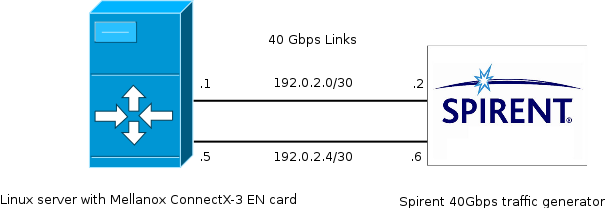
\includegraphics[width=13.5cm,keepaspectratio]{fig/net-setup.png}
	\caption{Measurement setup}
	\label{fig:measurements-setup}
\end{figure}


Enable IPv4 packet forwarding:
echo 1 > /proc/sys/net/ipv4/ip\_forward


ip neigh add 1.0.0.2 lladdr f4:52:14:5e:6c:71 dev enp6s0d1
ip neigh add 2.0.0.2 lladdr f4:52:14:5e:6c:70 dev enp6s0

ip addr add 1.0.0.1/24 broadcast 1.0.0.255 dev enp6s0d1
ip addr add 2.0.0.1/24 broadcast 2.0.0.255 dev enp6s0


Load BGP routes:
\begin{lstlisting}
Basic info: size of leaf: 40 bytes, size of tnode: 40 bytes.
Main:
        Aver depth:     2.43
        Max depth:      8
        Leaves:         503308
        Prefixes:       538739
        Internal nodes: 114430
          1: 58725  2: 26171  3: 14808  4: 7316  5: 4239  6: 2103  7: 1065  8: 2  17: 1
        Pointers: 995798
Null ptrs: 378061
Total size: 61373  kB
\end{lstlisting}


%=========================================================================
% (c) 2014, 2015 Josef Lusticky

\section{Software and firmware}
Base CentOS 7 was installed on the server.
The operating system features Linux kernel based on version 3.10 -
the installed version is 3.10.0-123.20.1.el7.x86\_64.
The operating system was updated with all updates available as of 1st May 2015.
The upstream kernel version 4.0.2 was additionally installed from the ELRepo repository~\cite{elrepo-kernel-ml}.

The Linux kernel detects the Mellanox ConnectX-3 EN card automatically and loads the mlx4\_core and mlx4\_en module.
The mlx4\_core module prints the detected PCI-Express link parameters to the kernel's message buffer.
The buffer can be viewed using the {\it{dmesg}} utility and its partial output is shown bellow:
\begin{lstlisting}[language=TeX]
mlx4_core 0000:06:00.0: PCIe link speed is 8.0GT/s, device supports 8.0GT/s
mlx4_core 0000:06:00.0: PCIe link width is x8, device supports x8
\end{lstlisting}
The mlx4\_core module further registers interrupts and prints the assigned IRQ numbers for each queue
to the kernel's message buffer:
\begin{lstlisting}[language=TeX]
mlx4_core 0000:06:00.0: irq 61 for MSI/MSI-X
mlx4_core 0000:06:00.0: irq 62 for MSI/MSI-X
...
mlx4_core 0000:06:00.0: irq 90 for MSI/MSI-X
\end{lstlisting}

The driver uses either MSI or MSI-X feature of the PCI-Express bus, as described in section~\ref{sec:40gbe-throughput}.
The MSI-X feature is used automatically if the system supports it, otherwise the adapter uses MSI.
The {\it{lspci -vv}} command can be used to check whether MSI-X is used.
Listing~\ref{lst:setup-lspci} shows partial output of lspci for the Mellanox ConnectX-3 EN adapter.
The MSI-X capability is followed by an Enable flag which is followed with either "+" (enabled)
or "-" (disabled).
Listing~\ref{lst:setup-lspci} shows that the system supports MSI-X and the adapter is configured to use it.
\begin{lstlisting}[language=TeX,label={lst:setup-lspci},caption={Partial output of lspci -vv for Mellanox ConnectX-3 EN}]
06:00.0 Ethernet controller: Mellanox Technologies MT27500 Family [ConnectX-3]
		...
		Capabilities: [9c] MSI-X: Enable+ Count=128 Masked-
				...
				LnkCap: Port #8, Speed 8GT/s, Width x8, ASPM L0s, Exit Latency L0s unlimited, L1 unlimited
				...
\end{lstlisting}

Apart from the NIC driver, the Mellanox ConnectX-3 adapter uses its own proprietary firmware.
The firmware was updated to version 2.32.5100, which is the latest version available as of 10th January 2015.
The firmware is not part of the Linux kernel and its update procedure is described in appendix~\ref{app:firmware}.


\section{Software settings}
Change the scaling governor for each CPU present in the system to performance (default is powersave):
\begin{lstlisting}
echo performance | tee /sys/devices/system/cpu/cpu[0-9]*/cpufreq/scaling_governor
\end{lstlisting}
Disable SELinux by editing SELINUX variable in /etc/sysconfig/selinux
(default is enforcing) and reboot the computer to apply:
\begin{lstlisting}
vi /etc/sysconfig/selinux
	SELINUX=disabled
reboot
\end{lstlisting}
%To disable the netfilter completely execute systemctl stop firewalld.
%If disabling the netfilter is not appropriate, flush all chains iptables -F,
%delete all user-defined chains iptables -X (which can be checked again by iptables -L).
Disable netfilter completely:
\begin{lstlisting}[language=TeX]
systemctl stop firewalld
systemctl disable firewalld  # do not execute firewalld on boot
\end{lstlisting}
Enable IPv6 on all interfaces (or at least on the forwarding interfaces):
\begin{lstlisting}
echo 0 > /proc/sys/net/ipv6/conf/all/disable\_ipv6
\end{lstlisting}
Enable IPv4 forwarding:
\begin{lstlisting}
echo 1 > /proc/sys/net/ipv4/ip\_forward
\end{lstlisting}
Enable IPv6 forwarding on all interfaces (or at least on the forwarding interfaces):
\begin{lstlisting}
echo 1 > /proc/sys/net/ipv6/conf/all/forwarding
\end{lstlisting}

IPv4 neighbours:
\begin{lstlisting}
ip neigh add 192.0.2.2 lladdr 00:10:94:00:00:01 dev enp6s0d1
ip neigh add 192.0.2.6 lladdr 00:10:94:00:00:02 dev enp6s0
\end{lstlisting}
IPv6 neighbours:
\begin{lstlisting}
ip -6 neigh add 2001:db8:1::2 lladdr 00:10:94:00:00:03 dev enp6s0d1
ip -6 neigh add 2001:db8:2::6 lladdr 00:10:94:00:00:04 dev enp6s0
\end{lstlisting}

Assign IPv4 addresses:
\begin{lstlisting}
ip addr add 192.0.2.1/30 broadcast 192.0.2.3 dev enp6s0d1
ip addr add 192.0.2.5/30 broadcast 192.0.2.7 dev enp6s0
\end{lstlisting}
Assign IPv6 addresses:
\begin{lstlisting}
ip -6 addr add 2001:db8:1::1/64 dev enp6s0d1
ip -6 addr add 2001:db8:2::5/64 dev enp6s0
\end{lstlisting}

%Additional system settings for a particular measurement are described.


%=========================================================================
% (c) 2014, 2015 Josef Lusticky

\chapter{Measurements}\label{chap:measurements}
The results presented in this thesis are based on the setup and basic settings described in chapter~\ref{chap:setup}.
The CentOS~7 operating system
was installed on the server with two Intel Xeon E5-2660 v3 CPUs
and Mellanox ConnectX-3 EN 40~Gbps ethernet adapter, as described in section~\ref{sec:analysis-hardware}.
Each measurement put the server under 60~seconds of constant unidirectional traffic load,
as described in section~\ref{sec:analysis-metodology}.
Unless stated otherwise,
the bandwidth use is configured in frames per second with a unit of margin 50~000.

\section{CentOS~7 distribution kernel 3.10.0-123}
The CentOS~7 distribution kernel version 3.10.0-123.20.1.el7.x86\_64
was used in the measurements presented in this section.

	%=========================================================================
% (c) 2014, 2015 Josef Lusticky

% FINAL
\subsection{Measurement 1 - default configuration - single IPv4 flow}
The first measurement shows the routing performance with
IP addresses assigned, IP forwarding enabled and Netfilter rules flushed.

The IP addresses were assigned as described in section~\ref{sec:setup-server}.
The IP forwarding was enabled by echoing "1" to the /proc/sys/net/ipv4/ip\_forward file and the Netfilter rules
were flushed using {\it{iptables -F}}, because the default rules do not allow forwarding.
\\
\\
\begin{tabular}{ | l | l | l | l | }
\hline
Frame size & \% of link & bandwidth & frame rate \\
\hline
64     &  0.59\% & 0.24~Gb/s & 350~000 \\
594    &  4.30\% & 1.72~Gb/s & 350~000 \\
1518   & 10.77\% & 4.31~Gb/s & 350~000 \\
AMS-IX &  5.33\% & 2.13~Gb/s & 350~000 \\
\hline
\end{tabular}

	
	%=========================================================================
% (c) 2014, 2015 Josef Lusticky

% FINAL
\subsection{Measurement 2 - default configuration - 32 IPv4 flows}
Since the Linux kernel scaling mechanisms described in section~\ref{sec:linux-scaling}
are based on processing each flow by a different CPU,
the routing performance of the default configuration was tested against 32 IPv4 flows.
\\
\\
\begin{tabular}{ | l | l | l | l | }
\hline
Frame size & \% of link & bandwidth & frame rate \\
\hline
64     &  2.69\% &  1.08~Gb/s & 1~550~000 \\
594    & 19.65\% &  7.86~Gb/s & 1~600~000 \\
1518   & 49.22\% & 19.69~Gb/s & 1~650~000 \\
AMS-IX & 24.34\% &  9.74~Gb/s & 1~600~000 \\
\hline
\end{tabular}
\\
\\
As expected, the scaling mechanisms help to increase the routing performance of the Linux kernel.
The scaling mechanisms perform better when forwarding larger frames.
This may be caused by differences in memory management allocations,
since the memory management is common for all CPUs present in the system.

	
	%=========================================================================
% (c) 2014, 2015 Josef Lusticky

% FINAL
\subsection{Measurement 3 - single IPv4 flow}
Unlike the previous measurements,
the following measurements use the complete setup described in section~\ref{sec:setup-server} to increase the throughput.
\\
\\
\begin{tabular}{ | l | l | l | l | }
\hline
Frame size & \% of link & bandwidth & frame rate \\
\hline
64     &  1.68\% &  0.67~Gb/s & 1~000~000 \\
594    & 12.28\% &  4.91~Gb/s & 1~000~000 \\
1518   & 30.76\% & 12.30~Gb/s & 1~000~000 \\
AMS-IX & 15.22\% &  6.09~Gb/s & 1~000~000 \\
\hline
\end{tabular}
\\
\\
The Linux kernel is able to forward 1~million IPv4 packets per second on a single core.
\\
The following partial output of the /proc/interrupts file shows the interrupt mapping:
\begin{lstlisting}
      ... CPU8  CPU9   CPU10 CPU11 CPU12  ...
178:  ...    0     0  255725     0     0  ...  enp129s0-0
179:  ...    0     0       0     0     0  ...  enp129s0-1
180:  ...    0     0       0     0     0  ...  enp129s0-2
181:  ...    0     0       0     0     0  ...  enp129s0-3
182:  ...    0     0       0     0     0  ...  enp129s0-4
183:  ...    0     0       0     0     0  ...  enp129s0-5
184:  ...    0     0       0     0     0  ...  enp129s0-6
185:  ...    0     0       0     0     0  ...  enp129s0-7
186:  ...    0     0       0     0     0  ...  enp129s0d1-0
187:  ...    0     0       0     0     0  ...  enp129s0d1-1
188:  ...    0     0       0     0     0  ...  enp129s0d1-2
189:  ...    0     0       0     0     0  ...  enp129s0d1-3
190:  ...    0     0       0     0     0  ...  enp129s0d1-4
191:  ...    0     0  313670     0     0  ...  enp129s0d1-5
192:  ...    0     0       0     0     0  ...  enp129s0d1-6
193:  ...    0     0       0     0     0  ...  enp129s0d1-7
\end{lstlisting}
All packets are assigned to a single queue, in this case the queue number 5 ({\it{enp129s0d1}} is the receiving interface).
The smp\_affinity files show that the Linux kernel
automatically assigned each interrupt to the CPUs 10-19 and 30-39.
\begin{lstlisting}
cat /proc/irq/178/smp_affinity_list
	10-19,30-39
cat /proc/irq/179/smp_affinity_list
	10-19,30-39
...
cat /proc/irq/193/smp_affinity_list
	10-19,30-39
\end{lstlisting}
The {\it{lscpu}} utility or the Intel Performance Counter Monitor can be used to
verify that the CPUs 10-19 and 30-39 are logical cores of the CPU in Socket 1.
The CPU in this socket is directly connected to the PCI-Express link, as shown in figure~\ref{fig:setup-supermicro-board}.
\\
\\
The {\it{perf}} utility can be used to list the functions utilising the CPU 10.
\begin{lstlisting}
perf top -C 10
  11.42%  [kernel]  [k] fib_table_lookup
   9.62%  [kernel]  [k] _raw_spin_lock
   6.65%  [kernel]  [k] mlx4_en_xmit
   4.84%  [kernel]  [k] memcpy
   4.03%  [kernel]  [k] mlx4_en_complete_rx_desc
   3.61%  [kernel]  [k] check_leaf.isra.7
   3.52%  [kernel]  [k] mlx4_en_free_tx_desc.isra.22
   3.42%  [kernel]  [k] mlx4_en_process_rx_cq
   3.16%  [kernel]  [k] mlx4_en_poll_tx_cq
   2.89%  [kernel]  [k] put_compound_page
   2.72%  [kernel]  [k] dev_queue_xmit
\end{lstlisting}
The kernel spends most of the time on FIB lookup, which is performed by the {\it{fib\_table\_lookup}} function described
in section~\ref{sec:linux-routing}, and on locking.
\\
\\
The following listing shows the cache utilisation on all CPUs present in the system.
\begin{lstlisting}[language=TeX]
 L3MISS: L3 cache misses
 L2MISS: L2 cache misses (including other core's L2 cache *hits*)
 L3HIT : L3 cache hit ratio (0.00-1.00)
 L2HIT : L2 cache hit ratio (0.00-1.00)
 L3CLK : ratio of CPU cycles lost due to L3 cache misses (0.00-1.00), in some cases could be >1.0 due to a higher memory latency
 L2CLK : ratio of CPU cycles lost due to missing L2 cache but still hitting  L3 cache (0.00-1.00)
 L3OCC : L3 occupancy (in KBytes)

 Core (SKT) | L3MISS | L2MISS | L3HIT | L2HIT | L3CLK | L2CLK |  L3OCC

   0    0     4052       23 K    0.83    0.26    0.19    0.18      120
   1    0       52     1542      0.97    0.14    0.03    0.17       80
   2    0       37     1458      0.97    0.14    0.02    0.17      200
   3    0       42     1489      0.97    0.14    0.02    0.13        0
   4    0       36     1460      0.98    0.15    0.02    0.16        0
   5    0      223     1695      0.87    0.22    0.00    0.00       80
   6    0        4      542      0.99    0.13    0.00    0.12       40
   7    0        4      539      0.99    0.12    0.00    0.12        0
   8    0        4      533      0.99    0.12    0.00    0.11        0
   9    0       20      589      0.97    0.10    0.02    0.11       40
  10    1     1179     2608 K    1.00    0.88    0.00    0.04      240
  11    1      129      586      0.78    0.11    0.16    0.13        0
  12    1        7      531      0.99    0.12    0.01    0.16        0
  13    1      446     2223      0.80    0.14    0.06    0.05       80
  14    1        7      531      0.99    0.14    0.01    0.12        0
  15    1        7      535      0.99    0.13    0.01    0.13        0
  16    1        6      534      0.99    0.13    0.01    0.12        0
  17    1       16      675      0.98    0.17    0.01    0.12        0
  18    1       10      534      0.98    0.13    0.01    0.12        0
  19    1       24      607      0.96    0.11    0.02    0.10        0
  20    0      175     1090      0.84    0.07    0.08    0.14        0
  21    0        9      598      0.98    0.13    0.01    0.18        0
  22    0       80      974      0.92    0.14    0.01    0.03        0
  23    0       10      583      0.98    0.13    0.01    0.10        0
  24    0       15      831      0.98    0.12    0.01    0.17        0
  25    0       41      582      0.93    0.13    0.03    0.11        0
  26    0        4      513      0.99    0.13    0.00    0.13        0
  27    0        5      534      0.99    0.13    0.01    0.14       40
  28    0        5      534      0.99    0.12    0.01    0.12       40
  29    0       34      659      0.95    0.12    0.03    0.12        0
  30    1      102      603      0.83    0.12    0.16    0.17       40
  31    1       12      627      0.98    0.34    0.01    0.15      120
  32    1       37      544      0.93    0.12    0.05    0.16        0
  33    1       11      584      0.98    0.13    0.01    0.16       40
  34    1        7      528      0.99    0.14    0.01    0.17       40
  35    1        8      541      0.99    0.16    0.01    0.17        0
  36    1        8      541      0.99    0.12    0.01    0.16        0
  37    1       11      541      0.98    0.13    0.02    0.17       40
  38    1       11      553      0.98    0.12    0.01    0.16        0
  39    1     2105     4296      0.51    0.65    0.13    0.03      480
-------------------------------------------------------------------------
 SKT    0     4852       40 K    0.88    0.21    0.03    0.05      640
 SKT    1     4143     2624 K    1.00    0.87    0.00    0.04     1080
-------------------------------------------------------------------------
 TOTAL  *     8995     2664 K    1.00    0.87    0.00    0.04      N/A
\end{lstlisting}
The CPU 10 is performing the work related to TCP/IP processing.
Most of the cache misses are L2 miss, but there are also L3 misses.
The number of L3 misses is greatly reduced by the Intel Data Direct I/O technology,
as described in section~\ref{sec:analysis-hardware}.
The L2 hit ratio is 88\%, while L3 hit ration is almost 100\%.
Other CPUs are in idle state, except for CPU~0, which is running the Intel PCM and prints the output.

	
	%=========================================================================
% (c) 2014, 2015 Josef Lusticky

% FINAL
\subsection{Measurement 4 - 32 independent IPv4 flows}
This measurement can be compared with Measurement~2, except that the {\it{irqbalance}} daemon is disabled.
Therefore, the IRQ mapping is left untouched in its default state.
\\
\\
\begin{tabular}{ | l | l | l | l | }
\hline
Frame size & \% of link & bandwidth & frame rate \\
\hline
64     &  1.26\% &  0.50~Gb/s & 750~000 \\
594    & 12.28\% &  4.91~Gb/s & 800~000 \\
1518   & 24.61\% &  9.84~Gb/s & 800~000 \\
AMS-IX & 15.22\% &  6.09~Gb/s & 800~000 \\
\hline
\end{tabular}
\\
\\
When forwarding IP packets from multiple IPv4 flows on a single CPU,
the routing performance of the Linux kernel drops by 20\% against forwarding a single IPv4 flow.
The following listing shows that
the packets are uniformly distributed among all hardware queues.
However, the interrupts are not distributed among CPUs.
\begin{lstlisting}
      ... CPU8  CPU9   CPU10 CPU11 CPU12  ...
178:  ...    0     0  474701     0     0  ...  enp129s0-0
179:  ...    0     0       0     0     0  ...  enp129s0-1
180:  ...    0     0       0     0     0  ...  enp129s0-2
181:  ...    0     0       0     0     0  ...  enp129s0-3
182:  ...    0     0       0     0     0  ...  enp129s0-4
183:  ...    0     0       0     0     0  ...  enp129s0-5
184:  ...    0     0       0     0     0  ...  enp129s0-6
185:  ...    0     0       0     0     0  ...  enp129s0-7
186:  ...    0     0  317322     0     0  ...  enp129s0d1-0
187:  ...    0     0  317648     0     0  ...  enp129s0d1-1
188:  ...    0     0  317231     0     0  ...  enp129s0d1-2
189:  ...    0     0  317384     0     0  ...  enp129s0d1-3
190:  ...    0     0  317114     0     0  ...  enp129s0d1-4
191:  ...    0     0  317291     0     0  ...  enp129s0d1-5
192:  ...    0     0  317190     0     0  ...  enp129s0d1-6
193:  ...    0     0  317964     0     0  ...  enp129s0d1-7
\end{lstlisting}
Each receive queue triggers roughly the same number of interrupts as in the previous measurement,
but overall the NIC triggers much more interrupts.
The kernel spends more time on running the interrupt service routine code.
Apart from servicing interrupts, the kernel must fetch the packets from different ingress queues,
which in turn may need additional locking.
\\
The following listing shows partial output of {\it{perf}}:
\begin{lstlisting}
perf top -C 10
  12.07%  [kernel]  [k] _raw_spin_lock
   8.68%  [kernel]  [k] fib_table_lookup
   5.01%  [kernel]  [k] mlx4_en_xmit
   4.63%  [kernel]  [k] mlx4_en_process_rx_cq
   3.64%  [kernel]  [k] __netif_receive_skb_core
   3.49%  [kernel]  [k] memcpy
   3.08%  [kernel]  [k] irq_entries_start
   2.68%  [kernel]  [k] mlx4_eq_int
   2.33%  [kernel]  [k] mlx4_en_poll_tx_cq
   2.24%  [kernel]  [k] ip_route_input_noref
\end{lstlisting}
The kernel spends most of the time on locking and FIB table lookup.

	
	%=========================================================================
% (c) 2014, 2015 Josef Lusticky

% FINAL
\subsection{Measurement 5 - single IPv4 flow over QPI}
Instruct the kernel to use the CPU~9 for processing the RX interrupts.
The softirq and forwarding code runs on CPU~9.
\begin{lstlisting}[language=TeX]
for i in `seq 178 193` ; do echo 9 > /proc/irq/\$i/smp_affinity_list ;done
\end{lstlisting}
The CPU~9 is not directly connected to the PCI-Express link with the NIC,
so QPI links between CPUs are used.

\begin{tabular}{ | l | l | l | l | }
\hline
Frame size & \% of link & bandwidth & frame rate \\
\hline
64     &  1.09\% &  0.44~Gb/s & 650~000 \\
594    &  7.98\% &  3.19~Gb/s & 650~000 \\
1518   & 19.99\% &  8.00~Gb/s & 650~000 \\
AMS-IX &  9.89\% &  3.96~Gb/s & 650~000 \\
\hline
\end{tabular}
The routing perfomance drops by 35\% when it is performed by
a CPU not directly connected to the PCI-Express link with the NIC.

\begin{lstlisting}[language=TeX]
 L3MISS: L3 cache misses
 L2MISS: L2 cache misses (including other core's L2 cache *hits*)
 L3HIT : L3 cache hit ratio (0.00-1.00)
 L2HIT : L2 cache hit ratio (0.00-1.00)
 L3CLK : ratio of CPU cycles lost due to L3 cache misses (0.00-1.00), in some cases could be >1.0 due to a higher memory latency
 L2CLK : ratio of CPU cycles lost due to missing L2 cache but still hitting  L3 cache (0.00-1.00)
 L3OCC : L3 occupancy (in KBytes)


 Core (SKT) | L3MISS | L2MISS | L3HIT | L2HIT | L3CLK | L2CLK |  L3OCC

   0    0     6209       24 K    0.75    0.32    0.19    0.12      480
   1    0       13      546      0.98    0.12    0.01    0.14      640
   2    0      154     4746      0.97    0.16    0.03    0.18       40
   3    0       16     1452      0.99    0.14    0.01    0.15        0
   4    0       68     1164      0.94    0.25    0.00    0.00       80
   5    0       10      537      0.98    0.13    0.01    0.14      160
   6    0        5      538      0.99    0.13    0.01    0.14        0
   7    0       10      543      0.98    0.12    0.01    0.13        0
   8    0       10      548      0.98    0.11    0.01    0.11        0
   9    0     2002 K   2798 K    0.28    0.74    0.20    0.02     2360
  10    1      790       12 K    0.94    0.14    0.08    0.24     4640
  11    1       29      985      0.97    0.12    0.02    0.15        0
  12    1       22      569      0.96    0.11    0.02    0.09        0
  13    1      325     2112      0.85    0.15    0.05    0.06       40
  14    1      238     1328      0.82    0.16    0.05    0.05      120
  15    1       28      526      0.95    0.16    0.02    0.07       40
  16    1       32      572      0.94    0.13    0.02    0.07        0
  17    1       27      563      0.95    0.11    0.02    0.08        0
  18    1       20      563      0.96    0.12    0.01    0.09       40
  19    1       30      606      0.95    0.11    0.02    0.09       40
  20    0      158     1017      0.84    0.07    0.08    0.13       40
  21    0       10      553      0.98    0.13    0.02    0.20        0
  22    0       10      739      0.99    0.10    0.01    0.16       40
  23    0        7      574      0.99    0.13    0.01    0.18        0
  24    0       10      578      0.98    0.14    0.01    0.16        0
  25    0        4      535      0.99    0.14    0.01    0.16        0
  26    0       11      551      0.98    0.12    0.01    0.16        0
  27    0       11      550      0.98    0.13    0.01    0.13        0
  28    0       10      560      0.98    0.13    0.01    0.14        0
  29    0       97     5729      0.98    0.07    0.00    0.05        0
  30    1      185      911      0.80    0.08    0.10    0.12        0
  31    1       19      572      0.97    0.11    0.02    0.13        0
  32    1       15      556      0.97    0.13    0.02    0.13       80
  33    1       23      591      0.96    0.13    0.02    0.12       40
  34    1       21      555      0.96    0.12    0.01    0.09        0
  35    1       21      539      0.96    0.15    0.02    0.09      120
  36    1       23      555      0.96    0.13    0.02    0.09        0
  37    1       63      684      0.91    0.18    0.01    0.02        0
  38    1       16      555      0.97    0.14    0.01    0.10        0
  39    1     4826     7108      0.32    0.52    0.24    0.02        0
------------------------------------------------------------------------
 SKT    0     2009 K   2844 K    0.29    0.73    0.20    0.02     3840
 SKT    1     6753       32 K    0.79    0.26    0.10    0.08     5160
------------------------------------------------------------------------
 TOTAL  *     2015 K   2877 K    0.30    0.73    0.19    0.02      N/A
\end{lstlisting}

CPU~9 performs the actual forwarding, while CPU~10
is busy with the QPI communication overhead.

\begin{lstlisting}
Intel(r) QPI data traffic estimation in bytes (data traffic coming to CPU/socket through QPI links):

               QPI0     QPI1    |  QPI0   QPI1  
----------------------------------------------------------------------------------------------
 SKT    0       90 M     90 M   |    0%     0%   
 SKT    1       70 M     71 M   |    0%     0%   
----------------------------------------------------------------------------------------------
Total QPI incoming data traffic:  323 M     QPI data traffic/Memory controller traffic: 0.39
\end{lstlisting}
Both QPI links are used.


perf top -C 9
\begin{lstlisting}
  21.25%  [kernel]  [k] _raw_spin_lock
  11.61%  [kernel]  [k] memcpy
   6.69%  [kernel]  [k] fib_table_lookup
   6.60%  [kernel]  [k] skb_gro_reset_offset
   4.55%  [kernel]  [k] udp_gro_receive
   3.96%  [kernel]  [k] mlx4_en_xmit
   3.44%  [kernel]  [k] mlx4_en_process_rx_cq
   2.93%  [kernel]  [k] mlx4_en_poll_tx_cq
\end{lstlisting}

perf top -C 10
\begin{lstlisting}
   9.77%  [kernel]  [k] find_busiest_group
   3.47%  [kernel]  [k] cpumask_next_and
   3.01%  [kernel]  [k] _raw_spin_lock
   2.93%  [kernel]  [k] ktime_get
   2.59%  [kernel]  [k] mlx4_en_DUMP_ETH_STATS
   2.58%  [kernel]  [k] run_timer_softirq
   2.36%  [kernel]  [k] idle_cpu
   2.22%  [kernel]  [k] __schedule
\end{lstlisting}

	
	%=========================================================================
% (c) 2014, 2015 Josef Lusticky

% FINAL
\subsection{Measurement 6 - 32 IPv4 flows with irqbalance daemon}
The measurement includes the {\it{irqbalance}} daemon enabled.
The {\it{irqbalance}} daemon is responsible for dynamically assigning the interrupts to CPUs
using the files found under /proc/irq/{\it{NUMBER}}/smp\_affinity,
as described in subsection~\ref{sub:analysis-settings-procfs}.
\\
\\
\begin{tabular}{ | l | l | l | l | }
\hline
Frame size & \% of link & bandwidth & frame rate \\
\hline
64     &  8.99\% &  3.60~Gb/s & 5~350~000 \\
594    & 68.15\% & 27.26~Gb/s & 5~550~000 \\
1518   & 98.50\% & 39.40~Gb/s & 3~202~210 \\
AMS-IX & 88.25\% & 35.30~Gb/s & 5~800~000 \\
\hline
\end{tabular}
\\
\\
The scaling mechanisms of the Linux kernel take advantage of interrupt assignment
done by the {\it{irqbalance}} daemon.
The server is able to route almost 36~Gbps of the simulated AMS-IX internet traffic.
The measurement further confirms that the scaling mechanisms are sensitive to the frame size.
The measurement featuring 1518~octet frames was configured to use 98.5\% of the link bandwidth.
\\
The following listing shows that the {\it{irqbalance}} daemon assigned IRQs to CPUs 11-18, 30 and 33-39.
The CPUs 12-19 are serving RX interrupts, while the CPUs 30-39 are serving TX interrupts
({\it{en29d1}} represents the receiving interface).

\newpage

\begin{landscape}
\vspace*{\fill}
\begin{lstlisting}
     CPU12 CPU13 CPU14 CPU15 CPU16 CPU17 CPU18 CPU19  CPU30  CPU33  CPU34  CPU35  CPU36  CPU37  CPU38  CPU39
178:     0     0     0     0     0     0     0     0      0 292448      0      0      0      0      0      0 en29-0
179:     0     0     0     0     0     0     0     0      0      0 292978      0      0      0      0      0 en29-1
180:     0     0     0     0     0     0     0     0      0      0      0 292698      0      0      0      0 en29-2
181:     0     0     0     0     0     0     0     0      0      0      0      0 286435      0      0      0 en29-3
182:     0     0     0     0     0     0     0     0      0      0      0      0      0 282449      0      0 en29-4
183:     0     0     0     0     0     0     0     0      0      0      0      0      0      0 288839      0 en29-5
184:     0     0     0     0     0     0     0     0      0      0      0      0      0      0      0 327901 en29-6
185:     0     0     0     0     0     0     0     0 325935      0      0      0      0      0      0      0 en29-7
186: 53145     0     0     0     0     0     0     0      0      0      0      0      0      0      0      0 en29d1-0
187:     0 53090     0     0     0     0     0     0      0      0      0      0      0      0      0      0 en29d1-1
188:     0     0 39978     0     0     0     0     0      0      0      0      0      0      0      0      0 en29d1-2
189:     0     0     0 40484     0     0     0     0      0      0      0      0      0      0      0      0 en29d1-3
190:     0     0     0     0 40072     0     0     0      0      0      0      0      0      0      0      0 en29d1-4
191:     0     0     0     0     0 39982     0     0      0      0      0      0      0      0      0      0 en29d1-5
192:     0     0     0     0     0     0 40488     0      0      0      0      0      0      0      0      0 en29d1-6
193:     0     0     0     0     0     0     0 43262      0      0      0      0      0      0      0      0 en29d1-6
\end{lstlisting}
\vspace*{\fill}
\end{landscape}

\noindent
\\
The listing bellow shows the cache use.
\begin{lstlisting}[language=TeX]
 L3MISS: L3 cache misses 
 L2MISS: L2 cache misses (including other core's L2 cache *hits*) 
 L3HIT : L3 cache hit ratio (0.00-1.00)
 L2HIT : L2 cache hit ratio (0.00-1.00)
 L3CLK : ratio of CPU cycles lost due to L3 cache misses (0.00-1.00), in some cases could be >1.0 due to a higher memory latency
 L2CLK : ratio of CPU cycles lost due to missing L2 cache but still hitting L3 cache (0.00-1.00)

 Core (SKT) | L3MISS | L2MISS | L3HIT | L2HIT | L3CLK | L2CLK |  L3OCC

   0    0     1076       11 K    0.91    0.17    0.01    0.01      120
   1    0      574     4139      0.86    0.12    0.10    0.14       40
   2    0      241     1421      0.83    0.18    0.12    0.12        0
   3    0      658       11 K    0.94    0.09    0.07    0.24        0
   4    0       19      580      0.97    0.14    0.02    0.12        0
   5    0       78      363      0.79    0.25    0.03    0.03        0
   6    0       65      710      0.91    0.15    0.04    0.10       40
   7    0       19      544      0.97    0.12    0.02    0.10       40
   8    0       13      648      0.98    0.11    0.01    0.08        0
   9    0       32      582      0.95    0.11    0.02    0.08        0
  10    1     1007     3598      0.72    0.06    0.72    0.37       40
  11    1     4452     3802 K    1.00    0.45    0.00    0.10       40
  12    1     4932     3770 K    1.00    0.42    0.00    0.10      240
  13    1     6273     4131 K    1.00    0.51    0.00    0.09       40
  14    1     5086     4211 K    1.00    0.52    0.00    0.09       80
  15    1     4762     4211 K    1.00    0.50    0.00    0.10       80
  16    1     4453     4111 K    1.00    0.54    0.00    0.09       80
  17    1     4680     4124 K    1.00    0.56    0.00    0.09      160
  18    1     4737     4275 K    1.00    0.48    0.00    0.10       80
  19    1      105      573      0.82    0.18    0.18    0.17        0
  20    0      170      979      0.83    0.06    0.07    0.10       40
  21    0       16      692      0.98    0.10    0.01    0.12        0
  22    0       12      570      0.98    0.12    0.01    0.13        0
  23    0       15      839      0.98    0.10    0.01    0.13        0
  24    0       13      532      0.98    0.16    0.02    0.14        0
  25    0       22      441      0.95    0.21    0.01    0.06        0
  26    0       14      540      0.97    0.14    0.02    0.13        0
  27    0        9      516      0.98    0.15    0.01    0.13        0
  28    0      268     2659      0.90    0.09    0.10    0.18       40
  29    0      239      916      0.74    0.15    0.10    0.06        0
  30    1     1238     2816 K    1.00    0.60    0.00    0.27      680
  31    1       54      560      0.90    0.25    0.09    0.19       80
  32    1     3416     9666      0.65    0.20    0.72    0.27       40
  33    1       14 K   3887 K    1.00    0.64    0.00    0.27      640
  34    1       16 K   3969 K    1.00    0.63    0.00    0.27      960
  35    1       15 K   3881 K    1.00    0.64    0.00    0.27      960
  36    1       14 K   3878 K    1.00    0.63    0.00    0.27      880
  37    1       14 K   3920 K    1.00    0.63    0.00    0.27      440
  38    1       17 K   4014 K    1.00    0.63    0.00    0.27      600
  39    1     2106     2853 K    1.00    0.60    0.00    0.28     1240
------------------------------------------------------------------------
 SKT    0     3553       41 K    0.91    0.13    0.01    0.03      320
 SKT    1      141 K     61 M    1.00    0.57    0.00    0.14     7360
------------------------------------------------------------------------
 TOTAL  *      144 K     61 M    1.00    0.57    0.00    0.14      N/A 
\end{lstlisting}
The measurement featuring 1518~octet frames is the first measurement saturating the 40~Gbps Ethernet connection.
Intel PCM can be used to monitor the PCI-Express utilisation:
\begin{lstlisting}
Skt | PCIe Rd (B) | PCIe Wr (B)
 0         5270 K          86 K
 1           11 G        5422 M
--------------------------------
 *           11 G        5422 M
\end{lstlisting}
The PCI-Express link could be saturated when forwarding bidirectional traffic
- the PCI-Express 3.0 x8 throughput is 7~876.8~MB/s as calculated in section~\ref{sec:40gbe-throughput}.
Note, that there seems to be a bug in Intel PCM related to displaying
the PCIe Read bandwidth - it always shows double the expected value (11~Gigabytes does not make sense).

	
	%=========================================================================
% (c) 2014, 2015 Josef Lusticky

% FINAL
\subsection{Measurement 7 - 32 IPv4 flows with manual IRQ affinity mappings}
While {\it{irqbalance}} mapped the interrupts inteligently, it is always worth checking the mappings.
The dynamic mappings made by the {\it{irqbalance}} daemon can change during the run-time, which may lead
to unpredictable perfomance drops.
\\
The following listing shows the interrupt mapping scheme used during this measurement.
Unlike the mapping assigned by the {\it{irqbalance}} daemon,
this mapping targets both RX and TX interrupts to 8 CPUs only.
Additionally, Transmission Packet Steering (XPS) mechanism was configured
to maps each exclusively to a single CPUs, as described in section~\ref{sec:linux-scaling}.
\begin{lstlisting}[language=TeX]
echo 1 > /proc/irq/default_smp_affinity     # mask for new registered irqs
echo 0 | tee /proc/irq/*/smp_affinity_list  # assign all IRQs to CPU 0

echo 18 > /proc/irq/177/smp_affinity_list   # assign mlx4-async IRQ to CPU 18

echo 10 > /proc/irq/178/smp_affinity_list   # enp129s0-0 IRQ to CPU 10
echo 11 > /proc/irq/179/smp_affinity_list
echo 12 > /proc/irq/180/smp_affinity_list
echo 13 > /proc/irq/181/smp_affinity_list
echo 14 > /proc/irq/182/smp_affinity_list
echo 15 > /proc/irq/183/smp_affinity_list
echo 16 > /proc/irq/184/smp_affinity_list
echo 17 > /proc/irq/185/smp_affinity_list   # enp192s0-7 IRQ to CPU 17

echo 10 > /proc/irq/186/smp_affinity_list   # enp192s0d1-0 IRQ to CPU 10
echo 11 > /proc/irq/187/smp_affinity_list
echo 12 > /proc/irq/188/smp_affinity_list
echo 13 > /proc/irq/189/smp_affinity_list
echo 14 > /proc/irq/190/smp_affinity_list
echo 15 > /proc/irq/191/smp_affinity_list
echo 16 > /proc/irq/192/smp_affinity_list
echo 17 > /proc/irq/193/smp_affinity_list   # enp192s0d1-7 IRQ to CPU 17

# clear XPS on both interfaces
echo "0" | tee /sys/class/net/enp192s0/queues/tx-*/xps_cpus
echo "0" | tee /sys/class/net/enp192s0d1/queues/tx-*/xps_cpus

# use the IRQ mask to assign XPS
cat /proc/irq/178/smp_affinity > /sys/class/net/enp129s0/queues/tx-0/xps_cpus
cat /proc/irq/179/smp_affinity > /sys/class/net/enp129s0/queues/tx-1/xps_cpus
cat /proc/irq/180/smp_affinity > /sys/class/net/enp129s0/queues/tx-2/xps_cpus
cat /proc/irq/181/smp_affinity > /sys/class/net/enp129s0/queues/tx-3/xps_cpus
cat /proc/irq/182/smp_affinity > /sys/class/net/enp129s0/queues/tx-4/xps_cpus
cat /proc/irq/183/smp_affinity > /sys/class/net/enp129s0/queues/tx-5/xps_cpus
cat /proc/irq/184/smp_affinity > /sys/class/net/enp129s0/queues/tx-6/xps_cpus
cat /proc/irq/185/smp_affinity > /sys/class/net/enp129s0/queues/tx-7/xps_cpus

cat /proc/irq/186/smp_affinity > /sys/class/net/enp129s0d1/queues/tx-0/xps_cpus
cat /proc/irq/187/smp_affinity > /sys/class/net/enp129s0d1/queues/tx-1/xps_cpus
cat /proc/irq/188/smp_affinity > /sys/class/net/enp129s0d1/queues/tx-2/xps_cpus
cat /proc/irq/189/smp_affinity > /sys/class/net/enp129s0d1/queues/tx-3/xps_cpus
cat /proc/irq/190/smp_affinity > /sys/class/net/enp129s0d1/queues/tx-4/xps_cpus
cat /proc/irq/191/smp_affinity > /sys/class/net/enp129s0d1/queues/tx-5/xps_cpus
cat /proc/irq/192/smp_affinity > /sys/class/net/enp129s0d1/queues/tx-6/xps_cpus
cat /proc/irq/193/smp_affinity > /sys/class/net/enp129s0d1/queues/tx-7/xps_cpus
\end{lstlisting}
The {\it{mlx4}} driver uses combined interrupts for RX and TX,
therefore each mapped CPU serves RX and TX interrupts for the same packets.
Such mapping should lead to a better cache utilisation than in the previous measurement.
\\
\\
\begin{tabular}{ | l | l | l | l |}
\hline
Frame size & \% of link & bandwidth & frame rate \\
\hline
64     &  8.99\% &  3.60~Gb/s & 5~350~000 \\
594    & 68.15\% & 27.26~Gb/s & 5~550~000 \\
1518   & 99.60\% & 39.40~Gb/s & 3~202~210 \\
AMS-IX & 88.25\% & 35.30~Gb/s & 5~800~000 \\
\hline
\end{tabular}
\\
\\
The throughput performance with manual IRQ mappings is equal to the mappings set by the {\it{irqbalance}} daemon.
The measurement was also configured to use 128, 256, 512, 768, 1024 and 1280~byte sized frames
and the following graph presents the results.
\begin{figure}[H]
	\centering
	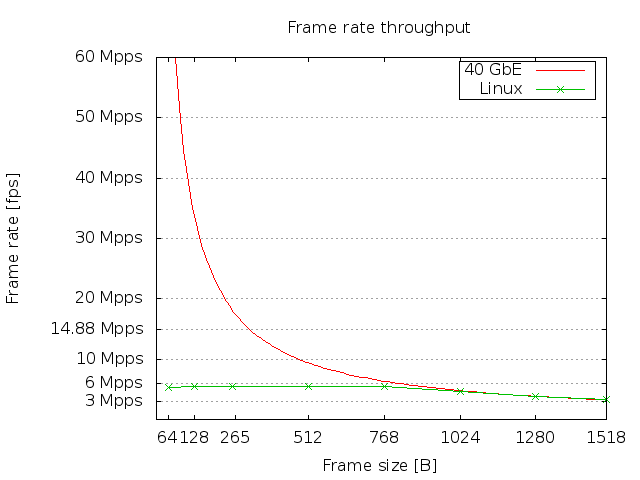
\includegraphics[width=12cm,keepaspectratio]{fig/frames.png}
\end{figure}
\noindent
The system is able to perform forwarding at nearly line rate speed with frames 1024~B and larger.
The following listing shows the actual interrupt mappings obtained from the /proc/interrupts file.
\newpage
%177:       0          0          0          0          0          0          0          0       1655  mlx4-async
\begin{landscape}
\vspace*{\fill}
\begin{lstlisting}
       CPU10      CPU11      CPU12      CPU13      CPU14      CPU15      CPU16      CPU17      CPU18
178:  298717          0          0          0          0          0          0          0          0  enp129s0-0
179:       0     294264          0          0          0          0          0          0          0  enp129s0-1
180:       0          0     291502          0          0          0          0          0          0  enp129s0-2
181:       0          0          0     296514          0          0          0          0          0  enp129s0-3
182:       0          0          0          0     302588          0          0          0          0  enp129s0-4
183:       0          0          0          0          0     294017          0          0          0  enp129s0-5
184:       0          0          0          0          0          0     294314          0          0  enp129s0-6
185:       0          0          0          0          0          0          0     302088          0  enp129s0-7
186:  402863          0          0          0          0          0          0          0          0  enp129s0d1-0
187:       0     411668          0          0          0          0          0          0          0  enp129s0d1-1
188:       0          0     416164          0          0          0          0          0          0  enp129s0d1-2
189:       0          0          0     422023          0          0          0          0          0  enp129s0d1-3
190:       0          0          0          0     421805          0          0          0          0  enp129s0d1-4
191:       0          0          0          0          0     415759          0          0          0  enp129s0d1-5
192:       0          0          0          0          0          0     402918          0          0  enp129s0d1-6
193:       0          0          0          0          0          0          0     413299          0  enp129s0d1-7
\end{lstlisting}
\vspace*{\fill}
\end{landscape}

\noindent
The RX and TX interrupts are spread across 8 CPUs.
The advantage of this mapping against the mapping done by the {\it{irqbalance}} daemon
is that it requires half the CPUs and the IRQ serving should cause fewer cache misses as well.
The listing bellow shows the cache statistics.
\begin{lstlisting}[language=TeX]
 L3MISS: L3 cache misses 
 L2MISS: L2 cache misses (including other core's L2 cache *hits*) 
 L3HIT : L3 cache hit ratio (0.00-1.00)
 L2HIT : L2 cache hit ratio (0.00-1.00)
 L3CLK : ratio of CPU cycles lost due to L3 cache misses (0.00-1.00)
 L2CLK : ratio of CPU cycles lost due to missing L2 cache (0.00-1.00)
 L3OCC : L3 occupancy (in KBytes)
 
 Core (SKT) | L3MISS | L2MISS | L3HIT | L2HIT | L3CLK | L2CLK |  L3OCC
   0    0     5799       33 K    0.82    0.24    0.19    0.18        0
   1    0      122     2488      0.95    0.15    0.03    0.14        0
   2    0      374     3928      0.90    0.19    0.00    0.00        0
   3    0        8      532      0.98    0.15    0.01    0.08       80
   4    0        6      519      0.99    0.16    0.00    0.08        0
   5    0       13      540      0.98    0.13    0.01    0.07        0
   6    0       12      552      0.98    0.14    0.01    0.07        0
   7    0       12      560      0.98    0.14    0.01    0.08      120
   8    0        9      547      0.98    0.13    0.01    0.08        0
   9    0       25      593      0.96    0.13    0.02    0.08        0
  10    1     9527     6014 K    1.00    0.51    0.00    0.14     1080
  11    1     9633     6096 K    1.00    0.52    0.00    0.14     1280
  12    1     9440     6257 K    1.00    0.53    0.00    0.15     1280
  13    1     9349     6069 K    1.00    0.54    0.00    0.14      960
  14    1     9147     6007 K    1.00    0.50    0.00    0.14     1000
  15    1     9270     6043 K    1.00    0.52    0.00    0.15     1160
  16    1     9382     6230 K    1.00    0.52    0.00    0.15     1560
  17    1     9249     6055 K    1.00    0.56    0.00    0.14      920
  18    1     1395     8002      0.83    0.15    0.29    0.29       40
  19    1      198     1129      0.82    0.12    0.13    0.14        0
  20    0      171     1042      0.84    0.08    0.07    0.11       40
  21    0       35     1176      0.97    0.16    0.02    0.17        0
  22    0       24      715      0.97    0.13    0.01    0.11       40
  23    0       18      537      0.97    0.15    0.01    0.09        0
  24    0        5      536      0.99    0.16    0.00    0.09        0
  25    0       11      533      0.98    0.14    0.01    0.08        0
  26    0       15      541      0.97    0.14    0.01    0.08        0
  27    0       11      538      0.98    0.16    0.01    0.09        0
  28    0       14      547      0.97    0.15    0.01    0.09        0
  29    0       46      672      0.93    0.12    0.03    0.10        0
  30    1      557     1200      0.54    0.34    0.03    0.01        0
  31    1      181      612      0.70    0.21    0.26    0.14       40
  32    1      192      604      0.68    0.23    0.25    0.12        0
  33    1      246      634      0.61    0.22    0.31    0.12        0
  34    1      202      622      0.68    0.22    0.28    0.15        0
  35    1      144      599      0.76    0.25    0.20    0.15        0
  36    1      127      620      0.80    0.22    0.17    0.15        0
  37    1      142      619      0.77    0.20    0.21    0.16       40
  38    1      132      685      0.81    0.11    0.13    0.15        0
  39    1      308      921      0.22    0.43    0.38    0.02      360
------------------------------------------------------------------------
 SKT    0     6730       50 K    0.87    0.21    0.03    0.04      280
 SKT    1       85 K     48 M    1.00    0.52    0.00    0.14     9720
------------------------------------------------------------------------
 TOTAL  *       92 K     48 M    1.00    0.52    0.00    0.14     N/A
\end{lstlisting}
As expected, the total cache miss count is lower with the manual IRQ mappings.
\\
The manual mappings are the best IRQ affinity settings in terms of number of CPUs used,
cache use and predictability.

	
	%=========================================================================
% (c) 2014, 2015 Josef Lusticky

% FINAL
\subsection{Measurement 8 - single IPv6 flow}

echo 0 > /proc/sys/net/ipv6/conf/all/disable\_ipv6
echo 1 > /proc/sys/net/ipv6/conf/all/forwarding
again, forwarding on only selected interfaces can be enabled.
ip6tables -F
ip6tables -X
ip6tables -L

ip -6 addr add 1::1/64 dev enp6s0d1
ip -6 addr add 2::1/64 dev enp6s0


%Single IPv6 flow.
%To test the difference between IPv4 and IPv6 routing lookup performance.

\begin{tabular}{ | l | l | l | l | }
\hline
Frame size & \% of link & frame rate \\
\hline
78     &  1.76\% &  0.71~Gb/s & 9~000~000 \\
594    & 11.05\% &  4.42~Gb/s & 9~000~000 \\
1518   & 27.68\% & 11.07~Gb/s & 9~000~000 \\
AMS-IX & 13.69\% &  5.48~Gb/s & 9~000~000 \\
\hline
\end{tabular}

perf top -C 14
\begin{lstlisting}
  11.75%  [kernel]  [k] ip6t_do_table
  10.37%  [kernel]  [k] _raw_spin_lock
   8.43%  [kernel]  [k] fib6_lookup
   4.93%  [kernel]  [k] ip6_forward
   3.66%  [kernel]  [k] fib6_get_table
   3.48%  [kernel]  [k] ip6_rcv_finish
   3.40%  [kernel]  [k] build_skb
   3.26%  [kernel]  [k] __netif_receive_skb_core
   3.01%  [kernel]  [k] mlx4_en_complete_rx_desc
   3.00%  [kernel]  [k] _raw_read_unlock_bh
   2.65%  [kernel]  [k] mlx4_en_process_rx_cq
   2.62%  [kernel]  [k] dst_release
\end{lstlisting}


	%=========================================================================
% (c) 2014, 2015 Josef Lusticky

% FINAL
\subsection{Measurement 9 - 32 IPv6 flows with manual IRQ affinity mappings}
The measurement can be directly compared to Measurement 7.
\\
\\
\begin{tabular}{ | l | l | l | l | }
\hline
Frame size & \% of link & bandwidth & frame rate \\
\hline
78     &  5.88\% &  2.35~Gb/s & 3~000~000 \\
594    & 36.84\% & 14.74~Gb/s & 3~550~000 \\
1518   & 98.50\% & 39.40~Gb/s & 3~202~210 \\
AMS-IX & 54.77\% & 21.91~Gb/s & 3~600~000 \\
\hline
\end{tabular}
\\
\\
The measurement featuring 1518~octet frames was configured to use 98.50\% of the link bandwidth.
The result shows a significant performance drop when routing multiple IPv6 flows.
\\
This performance drop can be investigated by changing the number of UDP flows to 8
and observing the interrupt distribution.
The following listing shows the partial output of the /proc/interrupts file when routing 8 flows.
\begin{lstlisting}
      ... CPU12 CPU13 CPU14 CPU15 CPU16 CPU17 CPU18 ...
 178: ...     0     0     0     0     0     0     0 ... enp129s0d1-0
 179: ...     0     0     0     0     0     0     0 ... enp129s0d1-1
 180: ...     0     0     0     0     0     0     0 ... enp129s0d1-2
 181: ...     0 32513     0     0     0     0     0 ... enp129s0d1-3
 182: ...     0     0     0     0     0     0     0 ... enp129s0d1-4
 183: ...     0     0     0     0     0     0     0 ... enp129s0d1-5
 184: ...     0     0     0     0     0     0     0 ... enp129s0d1-6
 185: ...     0     0     0     0     0 33543     0 ... enp129s0d1-7
 186: ...     0     0     0     0     0     0     0 ... enp129s0-0
 187: ...     0     0     0     0     0     0     0 ... enp129s0-1
 188: ...     0     0     0     0     0     0     0 ... enp129s0-2
 189: ...     0 19384     0     0     0     0     0 ... enp129s0-3
 190: ...     0     0     0     0     0     0     0 ... enp129s0-4
 191: ...     0     0     0     0     0     0     0 ... enp129s0-5
 192: ...     0     0     0     0     0     0     0 ... enp129s0-6
 193: ...     0     0     0     0     0 19576     0 ... enp129s0-7
\end{lstlisting}
In contrast to IPv4, the RSS does not distribute IPv6 packets uniformly.
As a result of this, the routing performance of IPv6 protocol is lower than in case of IPv4.
The traffic is also not distributed uniformly when routing 32 flows,
however, this issue cannot be detected from reading the /proc/interrupts file due to
interrupt mitigation mechanism used by NAPI, as described in subsection~\ref{sub:linux-ingress-napi}.


\section{Upstream mainline kernel 4.0.2}
The following measurements use the upstream Linux kernel downloaded form elrepo, as described in~\ref{sec:analysis-software}.
%This allows to use up to 16 queues with RSS.
%The Hyper-Threading must be enabled in order to have at least 16 cores.
%TODO 16 front + HT

	%=========================================================================
% (c) 2014, 2015 Josef Lusticky

%FINAL
\subsection{1 IPv4 flow}
\begin{tabular}{ | l | l | l | l | }
\hline
Frame size & \% of link & bandwidth & frame rate \\
\hline
AMS-IX & 15.22\% &  6.09~Gb/s & 1~000~000 \\
\hline
\end{tabular}
\\
\\
Routing performance of the Linux kernel version 4.0.2 on a single core is the same as the CentOS~7 distribution kernel 3.10.0-123.


\begin{lstlisting}
perf top -C 10
  11.25%  [kernel]            [k] _raw_spin_lock
   9.69%  [kernel]            [k] fib_table_lookup
   5.58%  [kernel]            [k] mlx4_en_xmit
   4.87%  [kernel]            [k] __memcpy
   4.65%  [kernel]            [k] mlx4_en_process_rx_cq
   2.98%  [kernel]            [k] put_compound_page
   2.73%  [kernel]            [k] __netif_receive_skb_core
   2.64%  [kernel]            [k] mlx4_en_poll_tx_cq
   2.43%  [kernel]            [k] ip_route_input_noref
   2.15%  [kernel]            [k] ip_rcv

\end{lstlisting}
FIB table lookup and locking take most of the time,
which is the same result as in case of the CentOS~7 distribution kernel.

	
	%=========================================================================
% (c) 2014, 2015 Josef Lusticky

% FINAL
\subsection{Single IPv6 flow}
\begin{tabular}{ | l | l | l | l | }
\hline
Frame size & \% of link & bandwidth & frame rate \\
\hline
78     &  1.67\% &  0.67~Gb/s & 850~000 \\
594    & 10.44\% &  4.18~Gb/s & 850~000 \\
1518   & 26.15\% & 10.46~Gb/s & 850~000 \\
AMS-IX & 12.93\% &  5.17~Gb/s & 850~000 \\
\hline
\end{tabular}

Kernel profiling:
\begin{lstlisting}
   9.43%  [kernel]  [k] _raw_spin_lock
   6.29%  [kernel]  [k] fib6_lookup_1
   5.49%  [kernel]  [k] mlx4_en_process_rx_cq
   4.12%  [kernel]  [k] mlx4_en_xmit
   3.62%  [kernel]  [k] memcpy
   3.09%  [kernel]  [k] mlx4_en_poll_tx_cq
   3.06%  [kernel]  [k] ip6_pol_route.isra.44
   2.84%  [kernel]  [k] irq_entries_start
   2.22%  [kernel]  [k] dst_release
   2.10%  [kernel]  [k] __netif_receive_skb_core
   2.08%  [kernel]  [k] __local_bh_enable_ip
   1.81%  [kernel]  [k] build_skb
   1.71%  [kernel]  [k] ip6_forward
   1.69%  [kernel]  [k] ipv6_rcv
\end{lstlisting}


	%=========================================================================
% (c) 2014, 2015 Josef Lusticky

% FINAL
\subsection{32 IPv4 flows on 16 queues}
The measurement uses the {\it{ethtool}} utility to configure the Mellanox ConnectX-3 EN adapter to use
16 receive queues per each port.
The network adapter supports up to 16 receive queues per port with RSS,
as described in section~\ref{sec:analysis-hardware}.
\begin{lstlisting}
ethtool -L enp129s0 rx 16
ethtool -L enp129s0d1 rx 16
\end{lstlisting}
The following table shows the result.
\\
\\
\begin{tabular}{ | l | l | l | l | }
\hline
Frame size & \% of link & bandwidth & frame rate \\
\hline
AMS-IX & 81.40\% & 32.56~Gb/s & 5~350~000 \\
\hline
\end{tabular}
\\
\\
Although the networking code runs on 16 logical CPUs simultaneously,
the performance is lower than in case of using 8 queues only.
This may be caused by the overhead of the Hyper-Threading technology.


	%=========================================================================
% (c) 2014, 2015 Josef Lusticky

% FINAL
\subsection{Single IPv6 flow}
The measurement can be directly compared to Measurement 8.
\\
\\
\begin{tabular}{ | l | l | l | l | }
\hline
Frame size & \% of link & bandwidth & frame rate \\
\hline
AMS-IX & 13.69\% &  5.48~Gb/s & 900~000 \\
\hline
\end{tabular}
\\
\\
The single flow routing performance is the same as in case of the CentOS~7 distribution kernel.
The following listing shows the output of the {\it{perf}} tool.
\begin{lstlisting}
perf top -C 10
   9.43%  [kernel]  [k] _raw_spin_lock
   6.29%  [kernel]  [k] fib6_lookup_1
   5.49%  [kernel]  [k] mlx4_en_process_rx_cq
   4.12%  [kernel]  [k] mlx4_en_xmit
   3.62%  [kernel]  [k] memcpy
   3.09%  [kernel]  [k] mlx4_en_poll_tx_cq
   3.06%  [kernel]  [k] ip6_pol_route.isra.44
   2.84%  [kernel]  [k] irq_entries_start
   2.22%  [kernel]  [k] dst_release
   2.10%  [kernel]  [k] __netif_receive_skb_core
   2.08%  [kernel]  [k] __local_bh_enable_ip
   1.81%  [kernel]  [k] build_skb
   1.71%  [kernel]  [k] ip6_forward
   1.69%  [kernel]  [k] ipv6_rcv
\end{lstlisting}


	%=========================================================================
% (c) 2014, 2015 Josef Lusticky

\subsection{32 IPv6 flows}
The measurement can be directly compared to Measurement 9.
\\
\\
\begin{tabular}{ | l | l | l | l | }
\hline
Frame size & \% of link & bandwidth & frame rate \\
\hline
AMS-IX & 54.77\% & 21.91~Gb/s & 3~600~000 \\
\hline
\end{tabular}
\\
\\
As in Measurement~9, the low performance is caused by the RSS distribution done by the network adapter.


\section{Settings influence}

	%=========================================================================
% (c) 2014, 2015 Josef Lusticky

% FINAL
\subsection{Disabled Hyper-Threading}
Routing of a single IPv4 flow was tested with the Hyper-Threading technology disabled.
\\
\\
\begin{tabular}{ | l | l | l | l | }
\hline
Frame size & \% of link & bandwidth & frame rate \\
\hline
64     &  1.93\% &  0.77~Gb/s & 1~150~000 \\
594    & 14.12\% &  5.65~Gb/s & 1~150~000 \\
1518   & 35.37\% & 14.15~Gb/s & 1~150~000 \\
AMS-IX & 17.50\% &  7.00~Gb/s & 1~150~000 \\
\hline
\end{tabular}
\\
\\
A single core routing performance increased by 15\% with disabled Hyper-Threading.
\\
Routing of 32 IPv4 flows with manual IRQ affinity mappings was tested to investiage
how is the routing performance influenced when the networking code runs
on multiple cores with Hyper-Threading disabled.
\\
\\
\begin{tabular}{ | l | l | l | l | }
\hline
Frame size & \% of link & bandwidth & frame rate \\
\hline
64     &  9.07\% &  3.63~Gb/s & 5~400~000 \\
594    & 68.77\% & 27.51~Gb/s & 5~600~000 \\
1518   & 98.50\% & 39.40~Gb/s & 3~202~210 \\
AMS-IX & 89.77\% & 35.91~Gb/s & 5~900~000 \\
\hline
\end{tabular}
\\
\\
Disabled Hyper-Threading provides only 2\% performance increase when routing the AMS-IX traffic on multiple cores.
The logical cores which are not utilised do not decrease performance significantly.
Hyper-Threading is highly optimised on Intel Xeon E5-2660 v3.


	%=========================================================================
% (c) 2014, 2015 Josef Lusticky

%FINAL
\subsection{Netdev\_budget}
The measurement increases the {\it{netdev\_budget}} NAPI parameter from its default 300 to 3~000.
The parameter is described in section~\ref{sec:linux-ingress}.
The {\it{netdev\_budget}} can be configured using {\it{procfs}}
\begin{lstlisting}
echo 3000 > /proc/sys/net/core/netdev_budget
\end{lstlisting}

\begin{tabular}{ | l | l | l | l | }
\hline
Frame size & \% of link & bandwidth & frame rate \\
\hline
AMS-IX & 88.25\% & 35.30~Gb/s & 5~800~000 \\
\hline
\end{tabular}
\\
\\
Increasing the {\it{netdev\_budget}} has no influence on routing performance,
which means that the raise softirq mechanism is highly optimised.


	%=========================================================================
% (c) 2014, 2015 Josef Lusticky

%FINAL
\subsection{Reverse path filter}
The measurement features Reverse path filter enabled, which is described in subsection~\ref{sub:analysis-settings-procfs}.
The rp\_filter can be enabled via {\it{procfs}}.
\begin{lstlisting}[language=TeX]
echo 1 | tee /proc/sys/net/ipv4/conf/*/rp_filter
\end{lstlisting}

\begin{tabular}{ | l | l | l | l | }
\hline
Frame size & \% of link & bandwidth & frame rate \\
\hline
AMS-IX & 55.54\% & 22.21~Gb/s & 3~650~000 \\
\hline
\end{tabular}
\\
\\
The rp\_filter introduces a significant performance drop of about 37\%.
The following listing shows the output of the {\it{perf}} utility.
\begin{lstlisting}
perf top -C 10
  39.88%  [kernel]  [k] fib_table_lookup
   8.35%  [kernel]  [k] check_leaf.isra.7
   6.43%  [kernel]  [k] _raw_spin_lock
   2.94%  [kernel]  [k] mlx4_en_xmit
   2.40%  [kernel]  [k] memcpy
   2.32%  [kernel]  [k] __netif_receive_skb_core
   2.18%  [kernel]  [k] mlx4_en_process_rx_cq
   2.14%  [kernel]  [k] fib_validate_source
   1.40%  [kernel]  [k] ip_route_input_noref
\end{lstlisting}
The {\it{fib\_table\_lookup}} is performed twice for each packet
and it is therefore taking much more of the CPU time.
There is also new {\it{fib\_validate\_source}} function, which calls
the actual {\it{fib\_table\_lookup}}.

In bidirectional routing with Reverse path filter enabled,
it may be worth changing the default RSS hash key to a symmetric one.
The RSS hash key is a taken as input by the Toeplitz hash function, as described in section~\ref{sec:linux-scaling}.
A symmetric RSS key would lead to processing both directions of the same flow on the same CPU,
therefore the result of the {\it{fib\_table\_lookup}} could be fetched from the CPU's cache~\cite{symetric-rss}.


	%=========================================================================
% (c) 2014, 2015 Josef Lusticky

%FINAL
\subsection{SELinux}
The measurement features enabled SELinux in Enforcing mode, which can be set in the {\it{/etc/sysconfig/selinux}} file.
\\
\\
\begin{tabular}{ | l | l | l | l | }
\hline
Frame size & \% of link & bandwidth & frame rate \\
\hline
AMS-IX & 80.64\% & 32.26~Gb/s & 5~300~000 \\
\hline
\end{tabular}
\\
\\
SELinux negatively impacts the routing performance by approx.~8.6\%.


	%=========================================================================
% (c) 2014, 2015 Josef Lusticky

\subsection{Firewall}
The measurement features enabled Netfilter and 10~000 filtering rules inserted.
The following commands were used to setup the measurement.
\begin{lstlisting}[language=TeX]
systemctl start firewalld
iptables -F
for i in `seq 10001 20000`; do iptables -A INPUT -p udp --dport $i -j DROP; done
\end{lstlisting}
The {\it{firewalld}} loads Netfilter modules automatically.
\begin{lstlisting}
lsmod | grep nf
nf_conntrack_ipv6      18738  5 
nf_defrag_ipv6         34651  1 nf_conntrack_ipv6
nf_nat_ipv6            13279  1 ip6table_nat
nf_conntrack_ipv4      14862  4 
nf_defrag_ipv4         12729  1 nf_conntrack_ipv4
nf_nat_ipv4            13263  1 iptable_nat
nf_nat                 21798  4 nf_nat_ipv4,nf_nat_ipv6,ip6table_nat,iptable_nat
nf_conntrack          101024  8 nf_nat,nf_nat_ipv4,nf_nat_ipv6,xt_conntrack,ip6table_nat,iptable_nat,nf_conntrack_ipv4,nf_conntrack_ipv6
\end{lstlisting}
The following table shows the results.
\\
\\
\begin{tabular}{ | l | l | l | l | }
\hline
Frame size & \% of link & bandwidth & frame rate \\
\hline
AMS-IX & 88.25\% & 35.30~Gb/s & 5~800~000 \\
\hline
\end{tabular}
\\
\\
The table above shows that 10~000 filtering rules have no impact on throughput.
The following listing shows the output of the {\it{perf}} utility.
\begin{lstlisting}
perf top -C 10
  16.37%  [kernel]  [k] fib_table_lookup
  11.48%  [kernel]  [k] _raw_spin_lock
   6.20%  [kernel]  [k] mlx4_en_process_rx_cq
   5.33%  [kernel]  [k] memcpy
   3.86%  [kernel]  [k] kmem_cache_alloc
   2.90%  [kernel]  [k] check_leaf.isra.7
   2.89%  [kernel]  [k] ipt_do_table
   2.57%  [kernel]  [k] mlx4_en_xmit
   2.42%  [kernel]  [k] mlx4_en_alloc_frags
\end{lstlisting}
The {\it{ipt\_do\_table}} function is responsible for the actual filtering.


	%=========================================================================
% (c) 2014, 2015 Josef Lusticky

\subsection{NAT}
The measurement features a simple Network Address Translation using Netfilter's {\it{MASQUERADE}},
which was configured using {\it{iptables}}.
\begin{lstlisting}
iptables -t nat -A POSTROUTING -o enp129s0 -j MASQUERADE

lsmod | grep nf
  nf_conntrack_ipv4      14862  1 
  nf_defrag_ipv4         12729  1 nf_conntrack_ipv4
  nf_nat_ipv4            13263  1 iptable_nat
  nf_nat                 21798  3 ipt_MASQUERADE,nf_nat_ipv4,iptable_nat
  nf_conntrack          101024  5 ipt_MASQUERADE,nf_nat,nf_nat_ipv4,iptable_nat,nf_conntrack_ipv4
\end{lstlisting}
The following table shows the results.
\\
\\
\begin{tabular}{ | l | l | l | l | }
\hline
Frame size & \% of link & bandwidth & frame rate \\
\hline
AMS-IX & 65.43\% & 26.17~Gb/s & 4~300~000 \\
\hline
\end{tabular}
\\
\\
The performance decreased by approx.~25\% when performing Network Address Translation using {\it{MASQUERADE}}.
Additionally, Netfilter provides other types of Network Address Translation such as {\it{SNAT}} or {\it{SAME}},
however, their description and performance comparison are outside the scope of this thesis.
The following listing shows the output of the {\it{perf}} tool.
\begin{lstlisting}
perf top -C 10
  12.71%  [kernel]  [k] fib_table_lookup
  10.84%  [kernel]  [k] _raw_spin_lock
   6.05%  [kernel]  [k] memcpy
   5.13%  [kernel]  [k] nf_xfrm_me_harder
   4.19%  [kernel]  [k] mlx4_en_process_rx_cq
   2.71%  [kernel]  [k] mlx4_en_xmit
   2.43%  [kernel]  [k] ip_route_input_noref
   2.14%  [kernel]  [k] nf_iterate
   2.07%  [kernel]  [k] check_leaf.isra.7
   2.02%  [kernel]  [k] __netif_receive_skb_core
\end{lstlisting}
The {\it{nf\_xfrm\_me\_harder}} function is responsible for the actual address translation.


\section{BGP routes}

	%=========================================================================
% (c) 2014, 2015 Josef Lusticky

The following measurement is perfomed with the Internet routes obtained from RIPE's BGP data.
The data contains 538~738 routes at the time of writing.
The complete setup of loading the routes into the kernel's FIB is described in appendix~\ref{app:bgp}.
The FIB statistics are exported via the {\it{/proc/net/fib\_triestat}} file, as described in
subsection~\ref{sub:analysis-metodology-collection}.
The following listing shows the content of the file after loading the Internet routes to the kernel's FIB.
\begin{lstlisting}
Basic info: size of leaf: 40 bytes, size of tnode: 40 bytes.
Main:
	Aver depth:     2.43
	Max depth:      8
	Leaves:         503308
	Prefixes:       538739
	Internal nodes: 114429
	  1: 58727  2: 26171  3: 14805  4: 7315  5: 4240  6: 2103  7: 1065  8: 2  17: 1
	Pointers: 995794
Null ptrs: 378058
Total size: 61373  kB

Counters:
---------
gets = 14129134
backtracks = 1913823
semantic match passed = 15973885
semantic match miss = 0
null node hit= 1360956
skipped node resize = 0

Local:
	Aver depth:     3.08
	Max depth:      4
	Leaves:         12
	Prefixes:       13
	Internal nodes: 7
	  1: 6  3: 1
	Pointers: 20
Null ptrs: 2
Total size: 2  kB

Counters:
---------
gets = 13959019
backtracks = 15201204
semantic match passed = 103193
semantic match miss = 0
null node hit= 8238092
skipped node resize = 0
\end{lstlisting}

\begin{tabular}{ | l | l | l | l | }
\hline
Frame size & \% of link & bandwidth & frame rate \\
\hline
AMS-IX & 77.60\% &  30.95~Gb/s & 5~100~000 \\
\hline
\end{tabular}

\begin{lstlisting}
 L3MISS: L3 cache misses 
 L2MISS: L2 cache misses (including other core's L2 cache *hits*) 
 L3HIT : L3 cache hit ratio (0.00-1.00)
 L2HIT : L2 cache hit ratio (0.00-1.00)
 L3CLK : ratio of CPU cycles lost due to L3 cache misses (0.00-1.00)
 L2CLK : ratio of CPU cycles lost due to missing L2 cache (0.00-1.00)
 L3OCC : L3 occupancy (in KBytes)

 Core (SKT) | L3MISS | L2MISS | L3HIT | L2HIT | L3CLK | L2CLK |  L3OCC

   0    0     4048       16 K    0.75    0.40    0.18    0.11      360
   1    0      574     3257      0.82    0.17    0.00    0.00      160
   2    0      515     4977      0.90    0.13    0.06    0.10       40
   3    0        5      539      0.99    0.11    0.00    0.12       40
   4    0        5      526      0.99    0.13    0.00    0.11        0
   5    0        5      532      0.99    0.12    0.00    0.10        0
   6    0        4      548      0.99    0.11    0.00    0.09        0
   7    0        4      541      0.99    0.12    0.00    0.09        0
   8    0        6      548      0.99    0.11    0.00    0.08       40
   9    0       21      550      0.96    0.13    0.01    0.07       40
  10    1     1410 K   9962 K    0.86    0.47    0.09    0.14     2480
  11    1     1400 K   9901 K    0.86    0.46    0.09    0.14     2160
  12    1     1396 K   9872 K    0.86    0.46    0.09    0.14     2200
  13    1     1396 K   9897 K    0.86    0.47    0.09    0.14     2000
  14    1     1402 K   9872 K    0.86    0.46    0.09    0.14     2720
  15    1     1395 K   9861 K    0.86    0.49    0.09    0.14     2160
  16    1     1409 K   9827 K    0.86    0.48    0.09    0.14     2200
  17    1     1402 K   9867 K    0.86    0.46    0.09    0.14     2240
  18    1      398      827      0.52    0.07    0.43    0.11        0
  19    1      200      891      0.78    0.07    0.08    0.09        0
  20    0      213      675      0.68    0.09    0.11    0.06        0
  21    0        7      656      0.99    0.09    0.01    0.13        0
  22    0        6      747      0.99    0.07    0.00    0.12       40
  23    0       13      548      0.98    0.12    0.01    0.12        0
  24    0        4      543      0.99    0.14    0.00    0.11       40
  25    0        5      529      0.99    0.13    0.00    0.10       80
  26    0       25      761      0.97    0.09    0.02    0.13        0
  27    0        5      707      0.99    0.09    0.00    0.12        0
  28    0        5      716      0.99    0.09    0.00    0.11        0
  29    0       45      643      0.93    0.11    0.03    0.09        0
  30    1      362      704      0.49    0.22    0.33    0.06       40
  31    1      206      643      0.68    0.21    0.24    0.12        0
  32    1      187      644      0.71    0.18    0.22    0.12        0
  33    1      188      635      0.70    0.38    0.24    0.13        0
  34    1      193      619      0.69    0.20    0.27    0.14        0
  35    1      208      614      0.66    0.11    0.34    0.15       40
  36    1      184      639      0.71    0.21    0.26    0.15        0
  37    1      194      642      0.70    0.19    0.26    0.13        0
  38    1      181      616      0.71    0.09    0.23    0.13        0
  39    1       22 K     29 K    0.24    0.16    0.85    0.06      200
------------------------------------------------------------------------
 SKT    0     5515       35 K    0.84    0.28    0.02    0.03       840
 SKT    1       11 M     79 M    0.86    0.47    0.09    0.14     18440
------------------------------------------------------------------------
 TOTAL  *       11 M     79 M    0.86    0.47    0.09    0.14     N/A
\end{lstlisting}




\chapter{Conclusion}
40Gbit software routing using GNU/Linux provides a reasonable alternative to expensive hardware routers.
The main bottleneck is. %TODO
 % viz. obsah.tex

  % Pouzita literatura
  % ----------------------------------------------
\ifczech
  \bibliographystyle{czechiso}
\else 
  \bibliographystyle{plain}
%  \bibliographystyle{alpha}
\fi
  \begin{flushleft}
  \bibliography{literatura} % viz. literatura.bib
  \end{flushleft}
  \appendix
  
  %=========================================================================
% (c) 2014, 2015 Josef Lusticky

\chapter{Populating kernel's FIB with BGP routes}\label{app:bgp}
RIPE Network Coordination Centre provides BGP data on its
website.\footnote{{\url{http://www.ripe.net/data-tools/stats/ris/ris-raw-data}}}
For the measurements in this thesis the data of RIPE NCC Amsterdam from 9th December 2014
The actual data can be obtained from the RIPE NCC's
site.\footnote{{\url{http://data.ris.ripe.net/rrc00/latest-bview.gz}}}

The BGP data is in MRT Routing Information Export Format, which is described in RFC~6396.
The data can be obtained from the Quagga routing daemon
using {\it{dump bgp routes}} command.
RIPE NCC provides bgpdump utility to parse this file to a human-readable text file.
To build bgpdump on CentOS 7 issue the following commands:
\begin{lstlisting}[language=TeX]
yum install bzip2-devel zlib-devel    # dependecies
wget http://www.ris.ripe.net/source/bgpdump/libbgpdump-1.4.99.13.tgz
tar xf libbgpdump-1.4.99.13.tgz
cd libbgpdump-1.4.99.13
./configure
make
make example     # needed prior make install
make install
\end{lstlisting}
Note that make example is required prior to make install.
Afterwards, bgpdump command should be avaliable (installed to /usr/local/bin/bgpdump).
The Makefile also supports make rpm target to generate rpm package (a wrong date in specfile needs to be corrected).

The bgpdump utility can parse the downloaded latest-bview.gz file directly (even wihout extracting first).
The following command extracts individual destination networks from the BGP data file and writes them to {\it{destinations}} file.
\begin{lstlisting}[language=TeX]
bgpdump latest-bview.gz | grep 'PREFIX' | grep '\.' | sed 's/PREFIX: \(.*\)/\1/' | uniq > destinations
\end{lstlisting}
The number of routes corresponds to the number of prefixes announced on the Internet.
Note that the first destination entry is default route 0.0.0.0/0 and the file also contains subnets such as 10.0.0.0/8 or 192.168.0.0/16,
which you may want to remove from the file prior to the next step.
Basically, you want to remove all the local routes from the generated file.
The local routes can be displayed using the following command.
\begin{lstlisting}[language=TeX]
ip route show table local | grep '^local'
\end{lstlisting}
If you are connected remotely, such as through SSH,
you must also remove routes to your local PC, which would break existing connection when misconfigured.
In case of the provided server's connection, the {\it{destinations}} file must not contain 195.113.0.0/16 prefix
The {\it{destinations}} file was obtained by running the following command:
\begin{lstlisting}[language=TeX]
bgpdump latest-bview.gz | grep 'PREFIX' | grep '\.' | sed 's/PREFIX: \(.*\)/\1/' | grep -v '195.113.0.0/16' uniq > destinations
\end{lstlisting}

The {\it{destinations}} file can be used to insert the router to the kernel's FIB table by ip route add command.
To insert subnets from the {\it{destinations}} file to the kernel's FIB, the following C program was written.
The neighbours of the local router, which are used to forward the packets, are specified in the {\it{gateways}} array.
This array needs to be adjusted prior to executing.
The destination subnets are then inserted to kernel's FIB via these neighbours.
The program takes a single argument, path to the {\it{destinations}} file generated as described above.
Note the {\it{execlp()}} function call on line 57, which performs the route insertions.
\begin{lstlisting}[numbers=left]
#include <stdio.h>
#include <stdlib.h>
#include <unistd.h>
#include <errno.h>
#include <sys/wait.h>

#if !defined(ARRAY_SIZE)
    #define ARRAY_SIZE(x) (sizeof((x)) / sizeof((x)[0]))
#endif

/* Define your gateway IP addresses */
char *gateways[] = { "192.0.2.6" }; //, "193.160.39.1" }; // , etc. };

int main(int argc, char *argv[])
{
  char *gw;
  char *buf;
  size_t size = 64;
  int i = 0;

  if (argc != 2)
  {
    fprintf(stderr, "Usage: %s dstfile\n", argv[0]);
    return EXIT_FAILURE;
  }

  FILE *f = fopen(argv[1], "r");
  if (f == NULL)
  {
    fprintf(stderr, "%s %d\n", argv[1], __LINE__);
    return EXIT_FAILURE;
  }

  buf = malloc(64);
  if (buf == NULL)
  {
    fprintf(stderr, "%s %d\n", argv[0], __LINE__);
    fclose(f);
    return EXIT_FAILURE;
  }

  ssize_t len;
  while ((len = getline(&buf, &size, f)) > 5) // get destination subnets
  {
    buf[len-1] = '\0';
    gw = gateways[i % ARRAY_SIZE(gateways)];
    pid_t pid = fork();
    if (pid == -1)
    {
      fprintf(stderr, "%s %d\n", argv[0], __LINE__);
      fclose(f);
      free(buf);
      return EXIT_FAILURE;
    }
    else if (pid == 0) // child
    {
      printf("ip route add %s via %s\n", buf, gw);
      execlp("ip", "ip", "route", "add", buf, "via", gw, NULL);
    }
    else // parent
    {
      wait(NULL); // wait for child
    }
    i++; // move to next gw
  }
  fclose(f);
  free(buf);
  return EXIT_SUCCESS;
}
\end{lstlisting}

The scripts and programs shown above can be found on the CD attached to this thesis.

\chapter{Updating the Mellanox ConnectX-3 EN firmware}\label{app:firmware}
The firmware can be updated using the Mellanox Firmware Tools (MFT), which can be downloaded
from the Mellanox management tools site.\footnote{{\url{http://www.mellanox.com/page/management_tools}}}
Installation of Mellanox Firmware Tools is described in MTF User Manual available at
the Mellanox documentation site.\footnote{{\url{http://www.mellanox.com/related-docs/MFT/MFT_user_manual.pdf}}}

The installation consists of unpacking the downloaded MFT archive and running the {\it{install.sh}} script.
This will install kernel-mft and mft packages.
The kernel-mft package contains required low-level kernel drivers, whereas the mft package contains utilities which use these drivers.
To start the Mellanox Software Tools service, which also loads the kernel drivers, run {\it{mst start}}.
Afterwards, the utilities from the mft package can be used, including the mlxfwmanager for updating the firmware.
The mlxfwmanager displays various information about the adapter, including the firmware version.

The newest firmware for the Mellanox ConnectX-3 adapters can be downloaded
from the Mellanox firmware site.\footnote{{\url{http://www.mellanox.com/page/firmware_table_ConnectX3EN}}}
Unzip the firmware and use the {\it{mlxfwmanager -u}} command in the same directory where the firmware was unzipped.
This will update the firmware.
After the update is complete, reboot is required to take effect.

Listing~\ref{lst:setup-firmware-update} shows the output of the firmware update procedure using the {\it{mlxfwmanager -u}} command.
The current firmware version is 2.31.5050, whereas the newer firmware placed in the current working directory is of version 2.32.5100.
The mlxfwmanager\_pci utility can be used to query the adapter information without starting the mst service.

\newpage

\begin{lstlisting}[language=TeX,label={lst:setup-firmware-update},caption={Firmware update procedure}]
[root@server]# mlxfwmanager -u
Querying Mellanox devices firmware ...

Device #1:
----------

  Device Type:      ConnectX3
  Part Number:      MCX314A-BCB_Ax
  Description:      ConnectX-3 EN network interface card; 40GigE; dual-port QSFP; PCIe3.0 x8 8GT/s; RoHS R6
  PSID:             MT_1090110023
  PCI Device Name:  /dev/mst/mt4099_pci_cr0
  Port1 MAC:        f452145e6c70
  Port2 MAC:        f452145e6c71
  Versions:         Current        Available     
     FW             2.31.5050      2.32.5100     
     PXE            3.4.0225       3.4.0306      

  Status:           Update required

---------
Found 1 device(s) requiring firmware update...

Perform FW update? [y/N]: y
Device #1: Updating FW ... Done

Restart needed for updates to take effect.
\end{lstlisting}

\chapter{General steps for maximum routing performance}\label{app:general-steps}
\begin{itemize}
\item the networking code does not benefit from Hyper-Threading, disable it
\item determine how many RX queues does the NIC support by "ethtool -{}-show-channels {\it{ifname}}" and use all of them using
"ethtool -{}-set-channels {\it{ifname}} rx {\it{num}}", beware that RSS usually limits addressing IRQs to power of 2 CPUs
\item disable {\it{irqbalance}} daemon and assign each IRQ exclusively to a single CPU via /proc/irq/{\it{NUMBER}}/smp\_affinity\_list
or /proc/irq/{\it{NUMBER}}/smp\_affinity
\item set the number of TX queues the same as RX queues by "ethtool -{}-set-channels {\it{ifname}} tx {\it{num}}" and assign exclusive mapping
of each queue to a single CPU
\item disable all daemons such as avahi, dbus, NetworkManager, etc.
\item check for disabled offloads by "ethtool -{}-show-offload {\it{ifname}}" and enable all of them
\item disable SELinux in /etc/sysconfig/selinux (and reboot to apply)
\item disable Netfilter if appropriate
\item set {\it{performance}} scaling governor for all CPUs
\item disable {\it{rp\_filter}} on all forwarding interfaces by writing "0" to \\
/proc/sys/net/ipv4/conf/{\it{ifname}}/rp\_filter,
beware that this might be required to set at boot time using the /etc/sysctl.conf file (use {\it{perf top}} to check)
\item avoid using DHCP and ARP/ND protocols, use static addressing and neighboring configuration instead
\end{itemize}
 % viz. prilohy.tex
\end{document}
